
%Documentclass thesul modifée pour la page de garde : thesul-cs
\documentclass[11pt]{thesul-cs}
\usepackage[utf8]{inputenc}
\usepackage[T1]{fontenc}
\usepackage{amsmath}
\usepackage{amsfonts}

%Fancy headers
\usepackage{fancyhdr}
\pagestyle{fancy}
\fancyhf{}
\fancyhead[LE,RO]{\thepage}
\fancyhead[LO]{\rightmark}
\fancyhead[RE]{\leftmark}

%mini table of contents
\usepackage[french]{minitoc}

\usepackage{amssymb}
\usepackage{xcolor} % où xcolor selon l'installation
\usepackage{mdframed}
\usepackage{multirow} %% Pour mettre un texte sur plusieurs rangées
\usepackage{multicol} %% Pour mettre un texte sur plusieurs colonnes
\usepackage{scrextend} %Forcer la 4eme  de couverture en page pair
\usepackage{tikz}
\usepackage{graphicx}
\usepackage[absolute]{textpos} 
\usepackage{colortbl}
\usepackage{amsmath}
\usepackage{amsthm}
\usepackage{array}
\usepackage{url}
\usepackage{algorithm2e}
\SetAlCapSkip{1em}
\SetKwInput{KwInput}{Input}
\SetKwInput{KwOutput}{Output}
\usepackage{mathtools}
\DeclareMathOperator{\sign}{sgn}
\newtheorem{propriete}{Propriété}
\newtheorem{proposition}{Proposition}

%draft/release options
\newif\ifDraft
\newcommand\comment[1]{\ifDraft {\itshape\color{red}{#1}} \fi} %text displayed in draft mode as comments
\newcommand\draft[1]{\ifDraft #1 \fi} %text displayed in draft mode only.

\newif\ifReview

%switch between draftmode and releasemode
\ifdefined\draftmode
  \Drafttrue
  %\Reviewtrue
\fi

\ifdefined\reviewmode
  \Reviewtrue
\fi


%\Drafttrue %switch to false if you want to get the release version.
%\Draftfalse %switch to true if you want to get the draft version.
\ifReview \usepackage[lmargin=5cm]{geometry}\fi
%def path for files


%---------------------------
% (1) Weights
%---------------------------
\newcommand\w{\omega}

%---------------------------
% (2) External inputs
%---------------------------
\newcommand\inpx{X}

%---------------------------
% (3) Contextual inputs
%---------------------------

\newcommand\inpc{\gamma}

%---------------------------
% (4) Contextual suffix
%---------------------------
\newcommand\cont{_{c}}

%---------------------------
% (5) External suffix
%---------------------------

\newcommand\ext{_{e}}

%---------------------------
% (6) Map index
%---------------------------
\newcommand\m[1]{^{({#1})}}

%---------------------------
% (7) BMU
%---------------------------

\newcommand\bmu{\Pi}

%---------------------------
% (8) Neighborhood radius
%---------------------------
\newcommand\h{h}

\DeclareMathOperator*{\argmax}{arg\,max}
\DeclareMathOperator*{\argmin}{arg\,min}

%compile only a chapter

\begin{document}
\dominitoc
\begin{titlepage}


%\thispagestyle{empty}

\newgeometry{left=7.5cm,bottom=2cm, top=1cm, right=1cm}

\tikz[remember picture,overlay] \node[opacity=1,inner sep=0pt] at (-28mm,-135mm){\includegraphics{Bandeau_UPaS.pdf}};

% fonte sans empattement pour la page de titre
\fontfamily{fvs}\fontseries{m}\selectfont


%*****************************************************
%******** NUMÉRO D'ORDRE DE LA THÈSE À COMPLÉTER *****
%******** POUR LE SECOND DÉPOT                   *****
%*****************************************************

\color{white}

\begin{picture}(0,0)

\put(-150,-735){\rotatebox{90}{NNT: 2020UPASA000}}
\end{picture}
 
%*****************************************************
%**  LOGO  ÉTABLISSEMENT PARTENAIRE SI COTUTELLE
%**  CHANGER L'IMAGE PAR DÉFAUT **
%*****************************************************
\vspace{-10mm} % à ajuster en fonction de la hauteur du logo
\flushright \includegraphics[width=0.4\textwidth]{CS.png}




%*****************************************************
%******************** TITRE **************************
%*****************************************************
\flushright
\vspace{10mm} % à régler éventuellement
\color{Prune}
\fontfamily{fvs}\fontseries{m}\fontsize{22}{26}\selectfont
 Auto-organisation décentralisée multi-cartes

%*****************************************************

%\fontfamily{fvs}\fontseries{m}\fontsize{8}{12}\selectfont
\normalsize
\vspace{1.5cm}

\color{black}
\textbf{Thèse de doctorat de l'Université Paris-Saclay}

\vspace{15mm}

École doctorale n$^{\circ}$ 000, dénomination et sigle\\
\small Spécialité de doctorat: voir annexe\\
\footnotesize Unité de recherche: voir annexe\\
\footnotesize Référent: : voir annexe
\vspace{15mm}

\textbf{Thèse présentée et soutenue à ....., le .... 202X, par}\\
\bigskip
\Large {\color{Prune} \textbf{Prénom NOM}}


%************************************
\vspace{\fill} % ALIGNER LE TABLEAU EN BAS DE PAGE
%************************************

\flushleft \small \textbf{Composition du jury:}
\bigskip



\scriptsize
\begin{tabular}{|p{8cm}l}
\arrayrulecolor{Prune}
\textbf{Prénom Nom} &   Président/e\\ 
Titre, Affiliation & \\
\textbf{Prénom Nom} &  Rapportrice \\ 
Titre, Affiliation   &   \\ 
\textbf{Prénom Nom} &  Rapporteur \\ 
Titre, Affiliation  &   \\ 
\textbf{Prénom Nom} &  Examinatrice \\ 
Titre, Affiliation   &   \\ 
\textbf{Prénom Nom} &  Examinateur \\ 
Titre, Affiliation   &   \\ 
\textbf{Prénom Nom} &  Examinateur \\ 
Titre, Affiliationt   &   \\ 

\end{tabular} 

\medskip
\begin{tabular}{|p{8cm}l}\arrayrulecolor{white}
\textbf{Prénom Nom} &   Directrice\\ 
Titre, Affiliation & \\
\textbf{Prénom Nom} &   Codirecteur\\ 
Titre, Affiliation  &   \\ 
\textbf{Prénom Nom} &   Coencadrante\\ 
Titre, Affiliation  &   \\ 
\textbf{Prénom Nom} &  Invité \\ 
Titre, Affiliation  &   \\ 


\end{tabular} 


\end{titlepage}
%%%%%%%%%%%%%%%%%%%%%%%%%%%%%%%%%%%%%%%%%%%%%%%%%%%%%%%%%%%%%%%
% 4eme de couverture
\ifthispageodd{\newpage\thispagestyle{empty}\null\newpage}{}
\thispagestyle{empty}
\newgeometry{top=1.5cm, bottom=1.25cm, left=2cm, right=2cm}
\fontfamily{rm}\selectfont

\lhead{}
\rhead{}
\rfoot{}
\cfoot{}
\lfoot{}

\noindent 
%*****************************************************
%***** LOGO DE L'ED À CHANGER ÉVENTUELLEMENT *********
%*****************************************************
\includegraphics[height=2.45cm]{IAEM}
\vspace{1cm}
%*****************************************************

\begin{mdframed}[linecolor=Prune,linewidth=1]
\vspace{-.25cm}
\paragraph*{Titre:} Auto-organisation décentralisée multi-cartes

\begin{small}
\vspace{-.25cm}
\paragraph*{Mots clés:} Cartes de Kohonen, Modularité, Architecture de réseaux de neurones

\vspace{-.5cm}
\begin{multicols}{2}
\paragraph*{Résumé:} 
\end{multicols}
\end{small}
\end{mdframed}

\begin{mdframed}[linecolor=Prune,linewidth=1]
\vspace{-.25cm}
\paragraph*{Title:} Multi-map decentralized self-organization

\begin{small}
\vspace{-.25cm}
\paragraph*{Keywords:} Kohonen maps, modularity, neural networks architecture

\vspace{-.5cm}
\begin{multicols}{2}
\paragraph*{Abstract:} 
\end{multicols}
\end{small}
\end{mdframed}

%************************************
\vspace{3cm} % ALIGNER EN BAS DE PAGE
%************************************
\fontfamily{fvs}\fontseries{m}\selectfont
\begin{tabular}{p{14cm}r}
\multirow{3}{16cm}[+0mm]{{\color{Prune} Université Paris-Saclay\\
Espace Technologique / Immeuble Discovery\\
Route de l’Orme aux Merisiers RD 128 / 91190 Saint-Aubin, France}} & \multirow{3}{2.19cm}[+9mm]\\
\end{tabular}
\tableofcontents
\chapter*{Introduction}

\subsection*{Réseaux de neurones artificiels et inspiration biologique}

1 - La biologie a été et est toujours une source d'inspiration pour les réseaux de neurones artificiels
    a - Le cerveau est une structure biologique implémentant des capacités de calcul exceptionnelles.
    b - Les réseaux de neurones actuels s'appuient sur une approche initialement biologique : perceptron, mais se sont concentrés sur des aspects computationnels.
    c - Cependant, de nombreux exemples montrent que l'inspiration biologique vient régulièrement apporter de nouveaux paradigmes alternatifs aux structures existantes.
    Par exemple, les réseaux de neurones impulsionnels ont été développés dans les années 90 mais apparaissent récemment comme une alternative moins énergivore aux réseaux de neurones classiques.
    Dans cet exemple, l'approche computationnelle et l'approche bio-inspirée se mêlent: on cherche à implémenter des réseaux de neurones classiques avec des SNN.
    d - Un enjeu plus ou moins actuel de l'inspiration biologique est la conception de réseaux de neurones autonomes, capable de mémoire et de prise de décision de façon non-supervisé. 
    Cet enjeu remonte déjà années 90 mais reste d'actualité encore aujourd'hui. 
    Une piste est s'inspirer de l'architecture du cerveau, présentant des modules interagissant entre eux. le comportement du cerveau est loin d'être compris, et de ce fait les possibilités d'inspiration biologiques peuvent être constamment revues.

=> cette thèse s'inscrit dans cette démarche d'architecture bio-inspirée.

2 - Architecture modulaire et émergence d'un comportement d'apprentissage

    a - La notion de modularité est présente en biologie, et notamment dans le cerveau : des zones fortement connectées sont liées entre elles par quelques connexions, induisant une notion de module d'un point de vue mésoscopique.
    b - Les systèmes modulaire régi par une dynamique présentent un comportement complexe : le comportement global émerge de l'interaction entre les éléments du système : il n'a lieu que parce que tous les éléments sont présents. Même si chaque élément peut être défini analytiquement, il nous faut simuler le système pour observer son comportement : il s'agit d'un système complexe.
    c -  d'un point de vue biologique, l'apprentissage à l'oeuvre dans le cerveau peut ainsi être défini comme un comportement émergent. Chaque neurone a des règles d'évolution simples, mais le comportement global du système résulte de l'interaction entre neurones.
    L'auto-organisation est une propriété émergent des systèmes biologique complexes.
    d-  D'un point de vue computationnel, l'émergence de comportements au sein d'architectures modulaires est une piste intéressante pour développer de nouvelles architectures et a été exploitée pour concevoir des réseaux utilisés aujourd'hui.
        - Réseaux de Hopfield
        - Automates cellulaires : présentent des capacité de calcul.
        - Deep Learning = interactions entre les couches 
        - Les DNF simulent des activités cérébrales, sans apprentissage. Lors de leur association et leur couplage, ils présentent cependant des comportements de prise de décision au sein du système. 

=>  On peut donc distinguer une démarche de création d'un système d'apprentissage qui part du but et décompose le problème en sous problèmes et d'entrainer des systèmes répondant à chacune des sous-taches, d'une démarche qui cherche à assembler des modules de même type afin d'en générer des comportements globaux. Cette deuxième approche a des résultats moins directement applicables que la première mais permet d'explorer des comportements alternatifs et est donc une source de recherche.
Cette thèse se place dans cette deuxième approche, vers la conception d'une architecture qui pourrait présenter des comportements émergents.

3 - Les SOMs, des modules possibles pour une architecture inspirée de la biologie
    a - Les cartes auto-organisatrices sont des exemples de modèles directement inspirés de l'organisation des aires cérébrales, mais s'étant computationnellement éloignées de la biologie pour faciliter les calculs, en remplacant par exemple le mécanismes de winner take all réalisé par des calculs locaux en un calcul d'argmax.
    b - propriétés : winner take all, auto-organisation = bonnes candidates pour les associer en architecture.
    c - De nombreux travaux ont cherché a associer les SOMs en architecture, mais peu de travaux ont exploré la construction d'une architecture générique modulaire présentant des rétroactions et éventuellement des connexions temporelles. 
    d- Les travaux précédents dans l'équipe ont associé des DNFs couplés à des SOMs afin d'ajouter un aspect apprentissage à ces réseaux. Les DNFs étaient alors utilisés pour le calcul d'activation des SOMs et leur couplage rétroactif engendrait une réponse dynamique des DNF qui évoluaient pour se stabiliser vers une position de consensus entre les Best Matching Unit des cartes. Les DNF sont en effet très proche des SOMs par leur notion de voisinage dans le calcul de l'activation, la relation avec la position dans l'espace des entrées et le mécanisme de Winner Take All, remplacé par un argmax dans une carte de Kohonen.

=> La thèse vise à utiliser des SOMs en tant que module d'une architecture, en introduisant un mécanisme de relaxation pour trouver des BMUs à une position de consensus dans l'architecture. 

4 - Un cadre d'étude possible : la mémoire associative 
    a - Le paragraphe 1 a présenté que les architectures modulaires vont vers la conception d'un système "cognitif" autonome concernant les réponses de l'architecture au système : traitement de données séquentielles, apprentissage sur le long terme sans oubli catastrophique des  données précédentes etc
    b - On peut décomposer ces objectifs en plusieurs aspects, notamment le coté temporel (récurrent) et l'aspect d'apprentissage multimodal : apprentissage de relations entre différents éléments sensoriels.
    Nous nous sommes concentrés dans cette thèse à l'étude des capacités d'apprentissage de l'architecture de cartes dans un contexte de mémoire associative.

5 - Problématique : 

Ces différents volets interdisciplinaires nous ont amené proposer un modèle d'architecture non-hiérarchique de carte auto-organisatrices que nous appelons CxSOM. Ce modèle 
Nos travaux cherchent ensuite à répondre à la problématique suivante~: 
Quels sont les comportements d'apprentissage émergeant de l'architecture CxSOM lors de tâches d'apprentissage de représentation d'entrée multimodales, et par quels mécanismes sont ils marqués lors du processus d'apprentissage ? 

6 - Plan de la thèse 




% Le terme calcul désigne les procédés abstraits utilisés pour le traitement de l'information. 
% Un système réalisant de tels procédés est alors désigné comme système de calcul. 
% D'un point de vue abstrait, ces systèmes peuvent ainsi être biologiques comme artificiels.
% Aussi de nombreux systèmes biologiques excellent à faire du calcul dès lors qu'ils interagissent avec leur environnement et s'adaptent à ce dernier~: 
% les réseaux mycellaires communiquent des informations au sein du réseau et échangent avec leur environnement~; les essaims d'abeilles sont capables de cartographier leur environnement grâce aux informations échangées entre individus. 
% Le blob est un être unicellulaire capable de s'étendre, qui est capable de résoudre des problèmes de recherche de plus court chemin, et ce seulement à partir de signaux chimiques circulant au sein de la cellule.
% Enfin, le cerveau est bien entendu un système de calcul~: il transforme une multitude de signaux physiques et chimiques provenant des capteurs du corps humain en activité électrique, dont émerge un apprentissage et des actions sur son environnement.
% Cette capacité d'apprentissage et surtout la recherche de son imitation est à l'origine du développement de l'intelligence artificielle et en particulier de l'apprentissage automatique, désignant les systèmes capable d'apprendre et de généraliser des informations à partir des données qui leur sont présentées.
% Les modèles d'apprentissage de Deep Learning les plus performants à l'heure actuelle s'appuient sur le perceptron, modèle inspiré à l'origine des neurones biologiques.
% La diversité des applications actuelles de l'apprentissage automatique et les méthodes de développement de ces algorithmes ont amené la recherche actuelle à se concentrer principalement sur les problèmes algorithmiques et computationnels que sur le développement de réseaux d'inspiration biologique.
% Cependant, la biologie, par sa diversité de comportements encore incompris, peut rester une inspiration dans le domaine des réseaux de neurones et apporte des paradigmes alternatifs pour la conception de structures d'apprentissage.
% Un exemple récent montrant le lien entre l'approche computationnelle et l'approche bio-inspirée se trouve dans les réseaux de neurones impulsionnels ou\emph{Spiking Neural Networks}. Ces réseaux sont directement inspirés du modèle biologique du neurone, et leur développement remonte à la fin des années 1980~\cite{Maass1996NetworksOS}.
% Ils apparaissent pourtant dans de nombreux travaux récents comme une méthode montante dans le domaine de l'apprentissage automatique pour la conception de modèles d'apprentissage moins énergivores et distribués. De nombreux travaux sur ces modèles de réseaux de neurones cherchent maintenant à adapter des réseaux de neurones classiques dans une version impulsionnelle. Il s'agit ici d'un exemple dans lequel l'inspiration biologique donne des alternatives possibles aux réseaux de neurones actuels et associent de façon complémentaire une approche bio-inspirée une approche plus computationnelle.
% D'un autre côté, les mécanismes à l'\oe{}uvre dans le cerveau restent loin d'être compris et modélisés.
% La question des calculs à l'\oe{}uvre dans les systèmes biologiques reste ainsi une thématique de recherche actuelle. 
% En ce sens, les découvertes de ces domaines sont des sources d'inspiration biologiques pertinentes.
% L'inspiration biologique cherche également à pl
% Nous plaçons cette thèse dans cette dynamique de recherche de réseaux de neurones inspirés de la biologie. Le but de ce domaine est d'étudier des mécanismes de calculs alternatifs qui pourront être intégrés et combinés à des approches plus classiques de conception de systèmes d'apprentissage, ou s'appliquer sur des applications robotiques.
% Une propriété globale des systèmes biologique tient dans la modularité et la non-hiérarchie des systèmes.
% On entend, par modularité d'un système sa composition en sous-systèmes autonomes effectuant des tâches différentes et collaborant entre eux. 
% Les systèmes modulaires présentent des avantages de réutilisation, de robustesse aux fautes, de redondance et de traitement local de l'information. Cette construction se retrouve dans les systèmes biologiques, \cite{clune_evolutionary_2013} proposant que ces avantages apportés par la modularité ont favorisé cette propriété lors de l'évolution.
% Cette de modularité est très générale. Nous pouvons en définir plusieurs aspects. 
% Des systèmes modulaires peuvent être composés de composants de structure différente interagissant entre eux. Un ordinateur est par exemple composé d'une multitude de modules spécifiques, conçus pour des tâches séparées et de structures complètement différentes.
% Un système modulaire peut également être composé de modules de même structure interagissant entre eux par des interfaces. 
% Par exemple, les colonies de fourmis sont composées d'individus de même structure.
% Les modules ont une fonction spécifique, qui peut être fournie a priori (fourmis guerrières/ouvrières) ou apprises par le module au cours de son interaction avec l'environnement.
% Si on s'intéresse au cerveau, ce dernier possède une structure a priori, mais le rôle de certaines aires cérébrales peut être redéfini et réappris au cours du temps~: l'aire visuelle d'un individu aveugle est réorganisée pour effectuer le traitement des autres sens de l'individu. 
% La modularité apporte alors une flexibilité au système.

% \subsection*{L'auto-organisation, une propriété bio-inspirée}

% Dans certains systèmes modulaires, le comportement dynamique global du système est souvent plus complexe que le comportement de chaque individu. 
% Lorsque c'est le cas, on parle de système complexe et le comportement global un comportement \emph{émergent} du système modulaire. Cette notion d'émergence, dont nous avons donné des exemples biologiques, a inspiré de nombreux modèles de calcul en intelligence artificielle et robotique.
% La fascination pour les comportements émergeant des systèmes complexes vient du fait que ce comportement global n'est analytiquement pas prévisible à partir des données des comportements élémentaires.
% Un exemple computationnel est l'étude des automates cellulaires dans le jeu de la vie. 
% Malgré des règles élémentaires simples, les automates présentes des capacités de mémoire et de transmission de donnée.
% L'intelligence d'essaim (swarm intelligence) est également une application directe du concept d'émergence à des sytèmes multi-agents qui interagissent localement avec leur environnement. 

% Ici encore, la cognition apparaît comme un comportement émergent de l'activité des neurones. Chaque neurone est construit sur le même modèle et les règles d'évolution de chaque neurone sont similaires. 
% Dans son ensemble, le cerveau présente des comportements de calculs qui lui sont propres.
% Dans ce même cerveau, à  une plus grande échelle, on peut séparer des zones fonctionnelles distinctes dans le cerveau. Chaque zone est de construction similaire, mais effectue une fonction différente.
% Le cerveau n'est pas le seul système biologique présentant ce type de fonctionnemment. Ainsi, les systèmes métaboliques ou d'expression de gènes sont des exemples de systèmes aggrégeant des éléments.
% Les colonies de fourmi sont constituées de milliers d'individus effectuants des actions à leur échelle et communiquant localement. Le comportement de la colonie est un système de calcul, capable de résoudre des problème d'optimisation de chemin vers une source de nourriture.

% Les réseaux biologiques hautement modulaires présentant cette capacité de traitement de l'information présentent également des propriétés d'auto-organisation; \cite{Siebert2020RoleOM} suggère même que la modularité est un élément clé pour la présence de motifs auto-organisés. 

% L'apprentissage est un exemple de comportement émergent d'un système. Perceptron multicouches comme comportement émergent de plusieurs couches.
% D'un point de vue modulaire, un exemple de système  = architectures de champs neuronaux dynamiques.
% Apparition de comportements complexes \cite{Sandamirskaya2014DynamicNF}


% \subsection*{Les cartes auto-organisatrices, un module bio-inspiré}

% Nous avons choisi dans cette thèse de s'intéresser à cette deuxième approche~: développer un système modulaire apprenant en associant des réseaux existants connus. 
% Nous nous intéressons spécialement aux cartes auto-organisatrices.

% Si nous revenons à un aspect biologique, les cartes auto-organisatrices sont, par leur comportement un modèle simplifié des aires cérébrales. Les travaux conduits dans notre équipe ces dernières années se sont attachés à construire des architectures modulaires complètement cellulaires. Nous cherchons dans cette thèse à s'inspirer de ces travaux mais en les passant à une échelle moins cellulaire, dans un cadre de simplification du modèle. Cette simplification nous permet une recherche plus facile et moins coûteuse de nouveaux comportements d'apprentissage, tout en restant déclinable si besoin en version cellulaire.
% Dans un cadre d'architecture modulaire,

% Les cartes auto-organisatrices et notamment le modèle de Kohonen sont largement utilisées en tant qu'algorithme d'apprentissage non supervisé appliqué à des tâches de réduction de dimension, de visualisation de données ou de classification.
% De nombreux travaux étudient l'utilisation de plusieurs cartes collaborant entre elles sur différentes applications, en général afin d'améliorer les performances de classification ou de regroupement de données d'une carte auto-organisatrice classique. Ces travaux se retrouvent sous le terme de SOM hiérarchiques, SOM multi-couches, ou \emph{Deep SOM}.
% Cependant, peu de travaux ont exploré l'aspect topologique et la simplicité des règles de calcul d'une carte pour les assembler en architectures modulaires comportant des rétroactions.
% Nous cherchons en plus à associer leur activité en un système dynamique, conférant à une architecture de cartes un comportement de prise de décision.

% L'étude d'une architecture non hiérarchique de cartes est d'une part motivée par leur inspiration biologique. Leur organisation rappelle en effet celle qu'on peut observer dans des aires cérébrales. Le cortex faisant apparaître des aires interagissant entre elles avec des boucles de rétroaction, la création d'une architecture non hiérarchique de cartes s'inscrit dans la continuité de cette inspiration biologique.
% Ensuite, l'étude des systèmes biologiques et la robotique sont liées~: la biologie sert d'inspiration à la robotique, que ce soit pour le mouvement d'un bras ou la prise de décision, et la robotique permet de tester des théories cherchant à modéliser des comportements biologiques \cite{Oudeyer2010OnTI}.
% Aussi les architectures de cartes bio-inspirées que nous avons relevées dans la littérature se placent aussi dans les domaines des neurosciences computationnelles ou de l'apprentissage incarné (\emph{Embodied intelligence}) en robotique \cite{Smith2005TheDO,cangelosi_embodied_2015}, à la frontière entre étude de la biologie et apprentissage automatique.

% Cette notion d'architecture modulaire de cartes est bien résumée par Kohonen dès 1995~:
% \begin{quote}
% Un objectif à long terme de l'auto-organisation est de créer des systèmes autonomes dont les éléments se contrôlent mutuellement et apprennent les uns des autres. De tels éléments de contrôle peuvent être implémentés par des SOMs spécifiques~; le problème principal est alors l'interface, en particulier la mise à l'échelle automatique des signaux d'interconnexion entre les modules et la collecte de signaux pertinents comme interface entre les modules. Nous laisserons cette idée aux recherches futures.
% \cite{Kohonen1995SelfOrganizingM}
% \end{quote}
% Ces éléments de contrôle sont les modules d'une architecture. 

% L'objectif de nos travaux est ainsi de proposer un modèle de carte qui puisse être utilisée en tant que module, de définir l'interface entre les modules afin de créer une architecture et de comprendre les comportements de calcul qui émergent de l'association des modules.


% Le chapitre 1 présente une zoologie des architectures de cartes de Kohonen existant dans la littérature.

\section*{Contributions et plan}

Cette thèse cherche donc, dans un cadre bio-inspiré, à construire une architecture modulaire décentralisée de cartes auto-organisatrices. L'idée de cette approche est de rechercher des nouveaux comportements d'apprentissage émergeant de l'interaction entre les modules d'une grande architecture, à l'inverse des méthodes plus ingénieures consistant à diviser une tâche connue en sous-systèmes.
Le manuscrit est organisé de la façon suivante.
Le chapitre~\ref{chap:archis} présente un état de l'art des architectures de cartes auto-organisatrices existantes afin de définir ce qu'on entend par architecture modulaire décentralisée et positionner notre modèle dans l'ensemble des modèles existants.
Nous détaillerons ensuite le modèle d'architecture décentralisée de cartes auto-organisatrices que nous proposons,CxSOM (\emph{Consensus-driven Multi-SOM}).
Ce modèle permet d'associer des cartes en architecture non-hiérarchiques. Dans ce modèle, les activités des cartes sont interdépendantes et l'apprentissage s'appuie sur une recherche de consensus entre les cartes pour la recherche d'un BMU, par un processus dynamique inspiré de la relaxation entre DNF.
Si le modèle a pour but à long terme de concevoir une architecture comportant de nombreux modules, nous avons concentré cette thèse sur l'analyse des comportements d'architecture de deux et trois cartes.
Le but de cette thèse est de proposer une méthodologie d'analyse de ce modèle et d'en tirer des comportements élémentaires.
Les expériences présentées dans la suite du manuscrit étudient le comportement de ces architectures sous différents points de vue.
Le chapitre~\ref{chap:relaxation} présente une analyse plus approfondie du mécanisme de relaxation permettant la recherche de BMUs entre cartes.
Nous proposerons ensuite une méthode expérimentale et des représentations rapprochant l'architecture de cartes de modèles d'apprentissage communs au chapitre \ref{chap:repr}.
Nous présenterons ensuite les comportements élémentaires observés sur des architectures de deux et trois cartes en une dimension, qui sont plus facile à visualiser. 
Nous présenterons notamment un comportement de prédiction rendu possible par le modèle.
Nous proposons au chapitre~\ref{chap:indicateur} des indicateurs numériques originaux d'évaluation de l'apprentissage associatif par l'architecture de cartes, dans le but d'étendre l'analyse du modèle à des architectures difficilement représentables visuellement.
Le chapitre é\ref{chap:analyse2D} utilise la méthodologie pour analyser le comportement d'architectures de cartes en deux dimensions afin de saisir la scalabilité du modèle.

Les travaux présentés dans cette thèse ont fait l'objet de deux présentations en conférence~:
\begin{itemize}
    \item Consensus driven ...., ICONIP 2020
    \item Input prediction in SOMs, ISCMI 2021
\end{itemize}

% A placer : 

% Apprentissage supervisé / non supervisé définition.
% Mémoire associative/traitement de séquences 


% \begin{itemize}
%     \item Apprentissage non supervisé, quantification vectorielle : définition + apprentissage développemental ? Pq c'est cool de continuer a etudier les SOM ?
%     \item Modularité et modularité dans les programmes informatiques,définition
%     \item Systèmes dynamiques complexes~: Biologique first puis exemple automates cellulaires qui sont une machine de turing, réseaux de Hopfields, machine de bolztmann: comporements de calcul comme émergeance
%     \item Systèmes d'apprentissage modulaire : des systèmes complexe.
% \end{itemize}

% \cite{Oudeyer2010OnTI} : biologie liée dans les deux sens à l'aspect computationnel.


% But : montrer comment un mécanisme de recherche de consensus entre cartes de Kohonen permet de construire des architectures apprenant des relations multimodales.

% \section{Comment construire un système modulaire d'apprentissage non supervisé}

% La modularité présente des aspects avantageux voire optimaux. 
% Une structure de réseau en petit monde est  utilisée dans des systèmes d'information, comme des bases de données, comme une structure optimisant la vitesse des échanges d'information dans le système. Or, ces structures sont également observées dans de nombreux domaines expérimentaux : biologie (exemple ?) et dans des systèmes sociaux tels que les arbres de connaissances entre individus. 

% D'un point de vue informatique, la modularité possède également de nombreuses définitions.
% On peut définir la modularité comme la décomposition d'un système en sous-systèmes plus petits et fonctionnant indépendamment. Ces systèmes interagissent via une interface bien définie.
% Plusieurs façons de construire ces sous-systèmes.
% Modules ayant des fonctions et structures différentes prédéfinie, exemple en programmation.
% Modules de même structure se différenciant au cours d'une interaction avec l'environnement (apprentissage). Dans ce cas de figure ces composants sont conçus pour être interchangeables et réutilisables.
% La modularité permet alors à un système d'être robuste à un dysfonctionnement d'un composant, sa mise à l'échelle et une faculté d'adaptation.

% Un système modulaire n'est pas forcément un système complexe.
% Cependant, lorsque l'interaction des modules est non linéaire, le système mène à l'émergence de nouveaux comportements.

% \section*{Modularité et Conception d'architectures d'apprentissage}

% Architecture d'apprentissage non supervisé = apprentissage de représentation. Passe par l'encodage de features de l'espace d'entrées sur des systèmes de calcul. 

% Les systèmes d'apprentissage existants combinent la notion de modularité et d'émergence pour former des comportements d'apprentissage plus complexes.
% Les réseaux de deep learning, se sont éloignés du modèle biologique du neurone pour ajouter des règles de calculs plus informatiques comme la backpropagation. Cependant l'approche modulaire est resté une constante dans le développement des réseaux utilisés actuellements comme le modèle teacher student et les réseaux de neurones adversarials qui combinent des réseaux performant chacun une sous-tâche par rapport à l'autre.

% La conception de système modulaire d'apprentissage peut passer par deux approches. D'un côté, une approche “finale” dans laquelle la finalité, l'application du système est connue. La conception du système passe alors par la décomposition de l'objectif en sous-systèmes et sous-tâches de manière à définir des modules particuliers.
% L'approche inverse serait l'approche constructive, dans laquelle nous disposons de modules permettant des comportements simples de calculs et les associons entre eux pour former un système modulaire. Il est difficile de connaître à l'avance le comportement final de ce type de système et son étude passe donc par la simulation.
% Cette approche, si elle n'est pas la plus directe en termes de résultats applicatifs, a l'avantage d'ouvrir la porte à des comportements d'apprentissages qui peuvent être inattendus. 

% Exemples d'archi modulaires d'apprentissage ?

% \subsubsection*{Mémoire associative et modularité}


% \subsection*{ Les cartes auto-organisatrices comme choix de modules : problématique de la thèse }
\mainmatter
\documentclass[../main]{subfiles}
\ifSubfilesClassLoaded{
    \dominitoc
    \tableofcontentsfile
}{}
\begin{document}

\graphicspath{{01-Modularite/},{./}}
%%%%%%%%%%%%%%%%%%%%%%%%%
% Intro du chapitre : Trouver un questionnement, un exemple qui parle de modularité dans les systèmes biologiques:  
% se placer dans le contexte de 
% - modularité : finalement on ne sait pas trop ce que c'est 
% - apprentissage ! 
% - réseaux de neurones
%%%%%%%%%%%%%%%%%%%%%%%%%
\chapter*{Introduction}


Le terme d'intelligence artificielle apparaît en 1956 lors d'une conférence donnée à l'université de Dartmouth, Dartmouth Summer Research Project on Artificial Intelligence. Cette conférence rassemble des chercheurs issus de différents domaines en plein essor de création comme la cybernétique, le traitement de l'information, la logique, la biologie, et veut poser les bases d'un nouveau domaine, nommé à cette occasion par les organisateurs Minsky et McCarthy: “Intelligence artificielle”. 

Ce terme générique est en fait large: on va appeler intelligence artificielle tout programme capable d'effectuer des tâches compliquées dont seuls les humains étaient initialement capables de résoudre. 
En terme d'architectures, les programmes d'intelligence artificielle peuvent être des systèmes figés à base de logique tels que les systèmes experts, ou des systèmes évolutifs. Parmi les tâches dites humaines se trouve en effet la notion d'apprentissage. La création  d'un système apprenant à partir d'entrées devient alors un enjeu à part entière de l'intelligence artificielle qu'on nommera apprentissage automatique ou en anglais machine learning.
Ces 60 dernières années ont alors vu les systèmes “intelligents” évoluer, se diversifier, pour résoudre de plus en plus de tâches jusqu'alors considérées comme humaines.

La conception de ces programmes passe par différentes sources d'inspirations, la biologie y prenant une place de premier choix.

\section*{Conception d'algorithmes d'apprentissage par modularité}

\subsection*{Définition de modularité}

La modularité en informatique se définit comme l'assemblage d'éléments séparés en une fonction globale, avec la condition qu'ajouter ou enlever un element ne modifie pas les autres éléments et influe seulement sur la fonction globale.

La majorité, voir tous les systèmes biologiques peuvent etre compris comme des systèmes modulaires. Il semble d'ailleurs que les systèmes modulaires sont privilégiés par l'évolution et des réseaux de forme similaire se retrouvent ainsi dans de nombreuses branches de la biologie: le cerveau présente des structures de réseau en petit monde que l'on retrouve dans l'organisation des ….
L'ingénieurie, sans même s'inspirer de la nature a recréé ces réseaux: les réseaux small world sont les plus efficaces pour la représentation de bases de données, ou la conception des réseaux aériens.
	
Cette notion de modularité concerne l'informatique en général: le concept peut etre appliqué au développement d'algorithmes.


\subsection*{Conception d'algorithmes d'IA}

La conception d'algorithme passe par piocher dans un ensemble de concepts et de fonctions connues, en les assemblant entre elles. 
La démarche de création d'algorithme peuvent etre ascendantes ou descendantes. 

Exemple d'algos d'IA → 
Ainsi, dans les années 1960, des premiers programmes d'intelligence artificielle repose sur des “micro mondes”, postulant qu'il est plus simple de décomposer les taches en taches plus simples afin de résoudre des comportements plus compliqués.

\subsection*{Approche ascendante vs approche descendantes}

On peut choisir deux axes de recherche pour développer un programme modulaire.
 L'approche descendante, la plus souvent utilisée, part du problème applicatif à résoudre pour le décomposer en probèmes-blocs plus simples.  et on estime que l'assemblage d'éléments exécutant ces fonctions simples nous permettrons d'effectuer la fonction complexe.
Cette démarche est très applicative. Elle est maitrisée: on connait la fonction finale, il suffit de trouver les meilleurs composants pour effectuer cette tache. Généralement, on a de bons résultats
Par contre, on ne pourra pas trouver de nouveaux paradigmes de calculs dans ce cadre: il s’agit plutot d’utiliser et d”appliquer des méthodes connues. 

Dans une démarche ascendante, il s’agit de partir de fonctions simples qu’on assemble dans l’idée d’en créer des complexes. Cette démarche est plutot exploratoire : la complexité du système fait que le seul moyen de comprendre le comportement du système ainsi créé est de le simuler. Cela peut etre vu comme un désavantage: pas possible d’avoir des équations et de choisir correctement les paramètres sans une étude des simulations. L’avantage par contre est de laisser de nombreuses opportunités ouvertes pour de nouvelles formes de calcul.
Et c’est précisément ce point qui nous amène à nous placer dans une telle démarche dans cette thèse. Nous voulons trouver de nouvelles formes de calcul pour faire de l’apprentissage. 

-----

\section*{ Modularité, systèmes complexes et emergence}

Un autre axe motivant notre reflexion sur des architectures modulaires d’apprentissage est l’observation que les systèmes modulaires sont des systèmes complexes. 

\subsection*{Système modulaire = système complexe ? }

Un système complexe est un système dont l'état est décrit par un certain nombre de variables qui évoluent de façon non linéaire. → def de qui ?
Dans la littérature, on rencontre également cette définition: système composé d'un grand nombre d'élements connectés entre eux. Cette définition rejoint la première, mais on peut noter qu'un système peut etre complexe meme à partir de 3 variables, tel que le modèle climatique de Lorentz ou le pendule triple.
 
La complexité d'un système est plutot un mode de représentation du système. La notion de systèmes complexes a été introduite dans les années 70 (Lorenz), et connait un essor depuis l'avenement des calculateur performants. 

Théorie des réseaux complexes

\subsection*{Emergence de calcul au sein d'un système complexe}

On va caractériser l'émergence de comportement dans un système complexe comme “le tout est plus que la somme des parties”, c'est à dire qu'on ne peut pas comprendre un système en le décomposant en éléments et en analysant chaque élémént individuellement: il va falloir considérer les relations entre éléments. 
La notion de systèmes complexe est étroitement liée à celle d'auto-organisation. La présence de patterns réguliers dans le comportement d'un système est directement liée à sa complexité.

\subsection*{Emergence de calcul comme moyen de conception de nouveaux algo d'IA}

D'un point de vue de création de systèmes, cela veut dire qu'on peut construire un système a partir d'éléments séparés, dont le comportement global résulte de l'interaction de ces éléments..
Le deep learning a été construit a partir du perceptron comme un assemblage de couches, dans le but de ????

\section*{ Plan de la thèse}

Dans cette thèse, nous voulons prendre une démarche constructive d'un algorithme d'apprentissage afin d'explorer de nouveaux paradigmes de calcul. Nous explorerons donc un système modulaire donc les modules sont des structures d'apprentissage existantes. Ce modèle dynamique est un système complexe, duquel pourra émerger des comportements
L'émergence de phénomènes d'auto organisation au sein des systèmes complexe nous pousse a considérer des modules possèdant déjà cette capacité d'auto-organisation: les cartes auto-organisatrices de Kohonen.
Le but de cette thèse est ainsi, dans une démarche constructive, de rechercher des nouveaux comportement d'apprentissage  à partir de cartes de Kohenen ,assemblées en architectures.
Nous nous intéressons à des modèles décentralisés, étant la clé pour construire n'importe quel type d'architecture par la suite. 
Cette démarche est difficile dans la mesure ou le comportement final d'une architecture n'est pas prédictible de prime abord. Tout l'exercice de cette thèse est alors de construire un modèle et définir des règles d'interaction, puis simuler et analyser ce modèle pour en tirer des comportements émergeants participant à l'apprentissage.
Dans cette démarche de construction, nous avons choisi des contraintes:
- Nous réalisons un système modulaire de cartes auto-organisatrices
- Cette architecture sera décentralisée: nous voulons permettre aux modules de communiquer avec n'importe lequel des autres éléments.
Le problème de cette thèse est d'étudier les comportements émergent de tels systèmes et d'étudier comment ces comportements sont un apprentissage des données.
Nous comparerons dans un premier chapitre les systèmes de cartes auto-organisatrices présentes dans la littérature et positionnerons l'architecture que nous développerons dans ce manuscrit au regard des travaux existants. Ces travaux nous permetterons de poser des hypothèses concernant le comportement qu'on peut attendre de l'architecture que nous développons. Nous présenterons ensuite le modèle CxSOM.
Nous définirons dans un chapitre la démarche expérimentale utilisée pour évaluer l'architecture de cartes et la représenter. Enfin, nous montrerons des comportements de base emergeant de la structure que nous avons développée et montrerons qu'elle a un capacité de mémoire associative. Nous présenterons egalement les limites du modèle. 
A l'issue du manuscrit, nous souhaitons que le lecteur aie une compréhension des comportements de base du modèle proposé, et aie des pistes pour l'utiliser de façon plus applicative.
\begin{figure}
    \begin{minipage}{0.49\textwidth}
        \includegraphics[width=\textwidth]{220px-Giant_Pufferfish_skin_pattern_detail}
    \end{minipage}
    \begin{minipage}{0.49\textwidth}
        \includegraphics[width=\textwidth]{turing_pattern_chem.pdf}
    \end{minipage}
\end{figure}
\end{document}







\chapter{Modèle d'architecture CxSOM}
\graphicspath{{02-SOM/}}
\minitoc

En réponse à la problématique de construire des architectures décentralisées de cartes de Kohonen, nous proposons dans cette thèse une version légèrement modifiée de carte auto-organisatrices, CxSOM. L'algorithme classique d'une SOM est modifié pour permettre à une carte de prendre plusieurs entrées; la recherche du BMU est également transformée.
Nous présentons dans cette partie l'algorithme CxSOM et les paramètres utilisés.

\section{Carte de Kohonen standard}\label{sec:kohonen}
L'algorithme CxSOM est directement dérivé de l'algorithme d'une carte de Kohonen classique \cite{kohonen92}. Le principe général d'une carte de Kohonen a été décrit dans le chapitre précédent; nous définissons ici plus précisément le modèle et les équations qui serviront de base pour la définition de l'algorithme CxSOM.
\subsection{Algorithme et notations}
Une carte de Kohonen est un graphe, généralement une ligne 1D ou une grille 2D de $N$ noeuds. Nous utiliserons dans cette thèse des cartes en une et deux dimensions, c'est à dire des lignes et des grilles. Les notations et le modèle présentés ici sont toutefois applicables à des cartes de dimension et topologies quelconques.

L'algorithme et les notations sont résumés en figure~\ref{fig:one_map_not}
Les entrées sont notées $\inpx_t$, tirées dans un espace d'entrée $D$. Le poids associé à un noeud est noté $\w_e \in D$. Sa \emph{position} dans la carte est indexée par $p$. Nous choisissons d'indexer les positions entre $0$ et $1$. L'ensemble des poids est noté ${\w_e(p), p \in [0,1]}$.
Une étape $t$ de l'algorithme de mise à jour d'une carte de Kohonen est le suivant:
\begin{enumerate}
\item\label{enum:inp} Une entrée $\inpx_t$ est présentée à la carte.
\item\label{enum:act} Une \emph{activité} $a_e(\inpx_t,p)$ est calculée dans la carte. 
Cette étape est déjà une légère modification souvent utilisée de l'algorithme de Kohonen. 
Dans la version classique, les distances entre l'entrée $\inpx$ et les poids $\w(p)$ sont considérées, et le BMU est l'unité dont le poids présente la plus petite distance à l'entrée. Ici, on prendra comme BMU l'unité correspondant au maximum de l'activité.
La fonction d'activité choisie est une activation gaussienne:
\begin{equation}\label{eq:act}
a_e(\inpx_t,p) = \exp{\frac{\lVert \inpx_t-\w\ext(p) \rVert ^2}{2\sigma^2}}
\end{equation}
\item\label{enum:bmu} L'unité ayant l'activité maximale est la \emph{Best Matching Unit} de la carte. Sa position est notée $\bmu$.
\item Chaque poids $\w_e$ est déplacé vers l'entrées $\inpx$. Le déplacement est pondéré par une \emph{fonction de voisinage} $h(\bmu,p)$, dépendant de la position de chaque unité dans la carte à la best matching unit. Elle est maximale en $p = \bmu$ et décroissante autour de cette position. Dans notre étude, la fonctions de voisinage est triangulaire, donc maximales en $\bmu$, décroissante sur le \emph{rayon de voisinage} $h_e$ et nulle sinon. Cela signifie que le BMU est déplacé vers l'entrée, et les poids des unités voisines du BMU dans un rayon $h_e$ sont également déplacés, mais selon un plus faible coefficient.
\begin{equation}
\w_e(p,t+1) = \w_e(p,t) + \alpha h(\bmu,p)(\inpx_t - \w_e(p,t))
\label{eq:update}
\end{equation}
\end{enumerate}


\begin{figure}
\centering
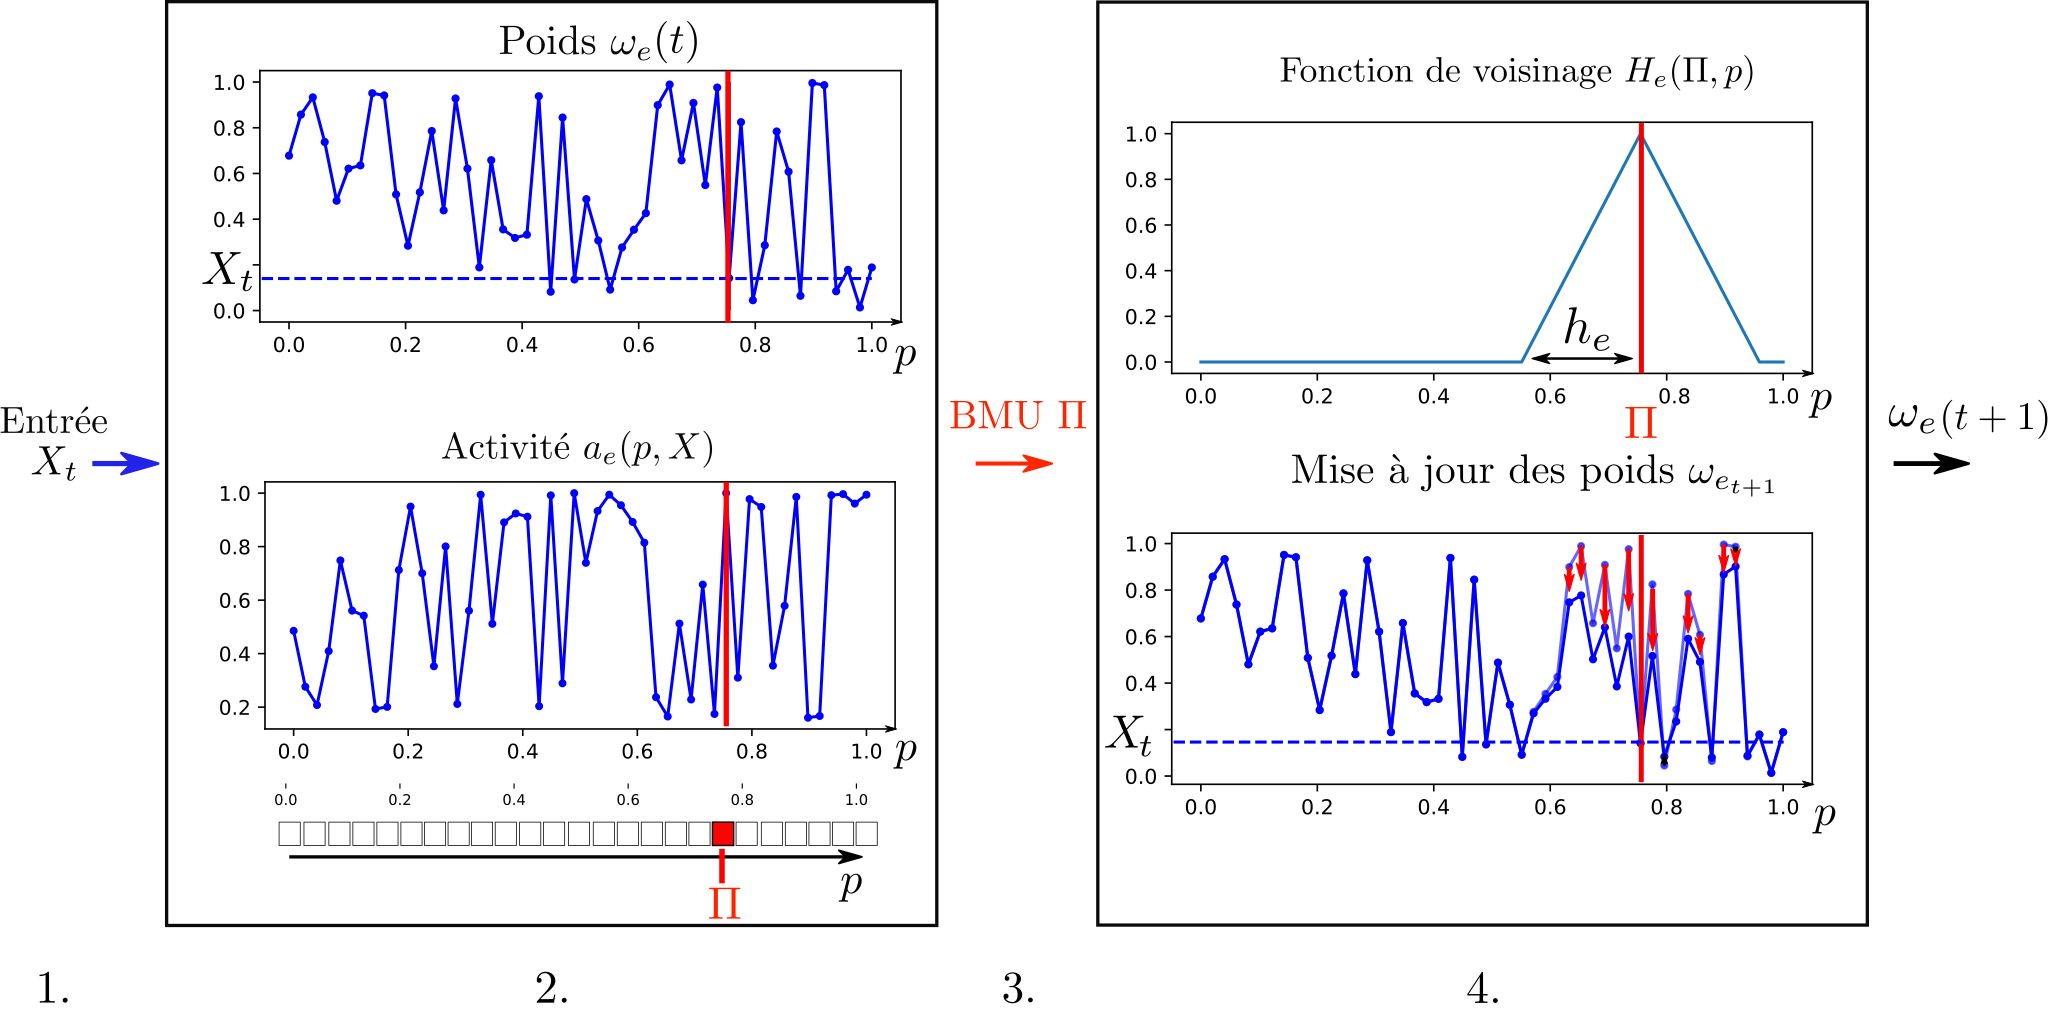
\includegraphics[width=\textwidth]{one_map_one_layer2.pdf}
\caption{Notations utilisées dans une carte de Kohonen simple}
\label{fig:one_map_not}
\end{figure}


\subsection{Paramètrage d'une carte de Kohonen}
Le dépliement d'une carte de Kohonen est géré par plusieurs paramètres. Nous détaillons ici les choix de paramètres effectués. 


\subsubsection{Taux d'apprentissage $\alpha$}

Le taux d'apprentissage $\alpha$ détermine la proportion dans laquelle chaque poids est déplacé vers l'entrée lors de sa mise à jour. Dans l'algorithme standard, le taux d'apprentissage décroit au cours de l'apprentissage. Au début de l'apprentissage, $\alpha$ est élevé, ce qui assure une organisation "grossière" rapide de la carte. $\alpha$ diminue ensuite de manière à cartographier plus localement les données. Cette décroissance assure principalement la convergence des poids de la carte au cours de l'apprentissage.
Dans l'algorithme CxSOM, nous utiliserons un taux d'apprentissage constant au cours de l'apprentissage. L'organisation des poids sera initialement un peu plus lente qu'une carte classique, mais cela permet de garder les paramètres constant au cours de l'apprentissage.
\comment{on n'aime pas les valeurs qui dépendent de $t$}
Nous observerons qu'en choisissant les bons paramètres, la convergence de la carte s'effectue correctement.
\subsubsection{Topologie de la carte}
Le graphe supportant la carte de Kohonen peut présenter diverses formes, comme détaillé en section\ref{sec:som001}. Les notations et l'algorithme CxSOM que nous présentons dans ce chapitre sont applicables à toutes les formes de cartes. Les expériences et l'évaluation du modèle se concentrent sur des lignes 1D et des grilles 2D, et omettent les formes de graphes quelconques. Ce choix est d'abord motivé par le fait que les lignes et les grilles étant les formats de cartes les plus courants rencontrés dans la littérature. On parle souvent de cartes 1D et cartes 2D lorsqu'on parle de cartes de Kohonen, en sous-entendant le format de ligne ou de grille du graphe support. Ces formes de cartes permettent de plus d'avoir une correspondance directe entre l'espace des positions $p \in [0,1]$ et un plan 1D ou 2D. Lorsqu'on parle de continuité dans une carte de Kohonen, il s'agit d'abord de proximité entre prototypes discrets. Le format de ligne et de grille permet d'étendre cette notion à une continuité des poids au sens mathématique, par interpolation. La carte est alors une fonction
\begin{equation*}
\begin{array}{ccccc}
M& : & [0,1]^2 \; \text{ou} \;[0,1] & \to & D \\
 & & p & \mapsto & \w_e(p) \\
\end{array}
\end{equation*}
Cette continuité est une des puissances d'une carte de Kohonen est est une de ses spécificité en tant qu'algorithme de quantification vectorielle. Dans le modèle CxSOM, nous traitons les positions $p$ comme un ensemble continu dans lequel faire des opérations.
Au cours de l'apprentissage, les poids d'une carte se rapprochent de la distribution des données, en gardant un ordre entre poids.
On parlera de \emph{dépliement} d'une carte pour parler de son apprentissage. Un exemple de dépliement d'une carte 1D sur des données 1D uniformément distribuées entre 0 et 1 est représenté en figure~\ref{fig:depliement}.
Dans ce cas, la carte 1D se rapproche de la fonction identité (ou moins l'identité): les poids sont ordonnés entre 0 et 1.
Ces deux configurations sont les deux seules considérées comme un bon apprentissage pour des cartes 1D sur des données 1D. Lorsque la dimension des données est plus grande que celle de la carte, par exemple des points 2D ou des images (256 dimension), la carte formera des plis de manière à remplir l'espace $D$. 

\begin{figure}
\centering
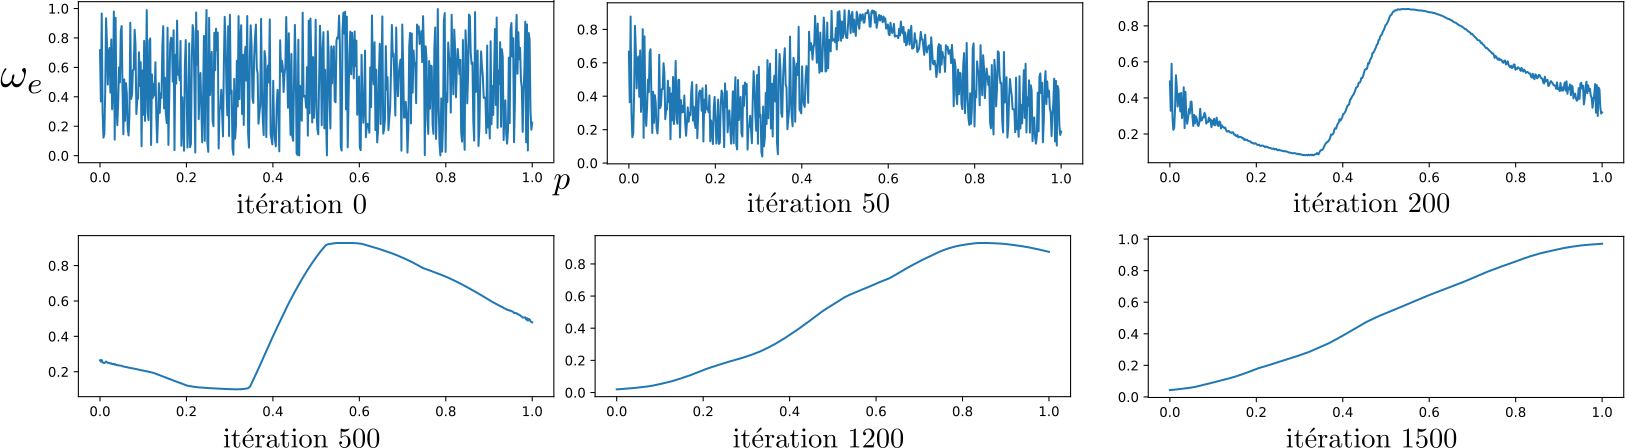
\includegraphics[width=\textwidth]{depliement_1D.pdf}
\caption{Exemple de dépliement d'une carte 1D de taille 500, sur des données 1D $\inpx \in [0,1]$. Les paramètres $h\ext = 0.2, \: \alpha = 0.2$ ont été gardé constants dans cet exemple. Une carte bien dépliée est assimilable à l'identité, comme sur cet exemple, ou moins l'identité. Ces configurations sont les deux seules pour lesquels les poids sont tous ordonnés suivant un ordre croissant ou décroissant.}
\label{fig:depliement}
\end{figure}

\subsubsection{Rayon de voisinage}
Le choix de la fonction de voisinage est déterminant dans la topologie de la carte, et en particulier le rayon de voisinage $h_e$.
Cette valeur détermine quelles unités voisines du BMU seront affectées par le déplacement du BMU.
Plus le rayon $h_e$ est grand, plus la partie de la carte déplacée vers l'entrée lors de la mise à jour est étendue. Un grand rayon d'apprentissage permet un dépliement plus rapide de la carte de Kohonen, mais l'apprentissage est peu précis car chaque poids est une moyenne d'un grand nombre de vecteurs. Les données déjà représentées sont rapidement oubliées par le déplacement des poids.
Un petit rayon d'apprentissage permet de déplacer les poids concentrés dans une petite région sans affecter toute la carte. Cela permet donc d'apprendre de nouvelles entrées sans oublier les parties déjà apprises. Par contre, utiliser un petit rayon de voisinage au début de l'apprentissage empêche une carte de bien se déplier et d'apprendre une structure globale des données. On doit donc trouver un compromis entre apprentissage de nouvelles données et mémoire des données déjà apprises.
Dans l'algorithme classique, ce compromis est trouvé en faisant décroitre le rayon de voisinage au cours de l'apprentissage. Un grand rayon de voisinage permet à la carte de se déplier rapidement en apprenant une structure globale des données. Sa décroissance permet d'affiner l'apprentissage des données à un niveau plus fin. 
Contrairement à la plupart des SOM classique, nous garderons des rayons de voisinage constants dans CxSOM. Ainsi, une étape de dépliement des cartes ne dépend pas de l'itération mais seulement de l'état précédent de la carte et de l'architecture.
%TODO citer des papiers recherchant un bon ensemble de paramètres pour l'algorithme de cartes auto-organisatrices.
\section{Modèle CxSOM}
A partir du modèle de carte de Kohonen détaillé en section \ref{sec:kohonen}, nous proposons une version de carte auto-organisatrice servant de bloc de base pour construire des architectures non-hiérarchique de cartes. Nous présentons dans cette section le modèle CxSOM. Toutes les notations et l'algorithme sont résumés en figure \ref{fig:one_map} et \ref{algo:cxsom}.

\subsubsection{Nombre de neurones d'une carte}
Le nombre de neurones d'une carte définit le niveau de quantification qu'on souhaite effectuer. Pour des opérations de classification, on choisira un nombre de neurones plus élevé que le nombre de classes, afin de pouvoir avoir plusieurs prototypes par classe.
Dans cette thèse, nous utilisons des cartes 1D comportant 500 noeuds. Le nombre de noeud est assez élevé pour pouvoir bien cartographier des ensembles de plus grande dimension. Ce nombre de noeud est proche de ce qu'on peut trouver dans la littérature.

\subsection{Choix généraux de développement}

Le modèle CxSOM étudié dans cette thèse doit permettre de construire des architectures \emph{non-hiérarchiques}. On souhaite que ce modèle soit générique, applicable à n'importe quel type d'architecture, et pouvant intégrer des connexions récurrentes. De cette manière, on ne se place pas dans une optique d'application précise mais de nouveau type de calcul. De nombreux modèles pourront être développés à partir de cette méthode. 


On définit une \emph{architecture} de carte un modèle composé de plusieurs modules qui sont chacun des cartes de Kohonen, et dans lequel des connexions sont définies entre ces éléments. Ces connexions ont un sens: on parle d'une connexions d'une carte A vers une carte B.
Dans une architecture, on peut construire un graphe $G$ orienté, dont les noeuds sont des cartes. La connexion d'une carte A vers une carte B est indiquée par la présence d'une arête de A vers B. On appelle architecture \emph{non-hiérarchique} une architecture pour laquelle $G$ n'est pas un arbre: il présente des boucles. Un exemple d'arhcitecture non-hiérarchique est représenté en figure~\ref{fig:archi_non_hierarchique}. Certaines cartes sont connectées dans les deux sens, d'autres en boucle.


Nous avons vu au chapitre précédent la notion de contexte transmise entre cartes. Dans CxSOM, on choisit de se placer dans le paradigme de transmission de la position du BMU entre cartes: on connecte une carte B à une carte A en donnant la position du BMU de B en entrée à la carte A. 
Ce paradigme de partage de positions a été utilisé dans le modèle hiérarchique HSOM~\cite{lampinen_clustering_1992}, et dans les modèles de cartes récurrentes s'appuyant sur SOMSD \cite{hammer_recursive_2004,hagenbuchner_self-organizing_2003,fix20}. Ces travaux montrent que la seule transmission d'une position de BMU permet 


L'utilisation du BMU comme contexte transmis est le paradigme choisi pour CxSOM. Contrairement aux cartes hiérarchiques HSOM dans lesquelle la position du BMU est la seule entrée d'une carte de plus haut niveau, chaque carte de l'architecture peut posséder une entrée principale propre, l'entrée \emph{externe}. L'entrée ou les entrées correspondant aux positions des BMUs d'autres cartes sont considérées comme une entrées supplémentaires d'une carte. Les cartes de Kohonen prennent donc un nombre arbitraire d'entrées, dont certaines sont les BMUs d'autres cartes. On appelle ces entrées internes à l'architecture les entrées \emph{contextuelles} d'une carte.
L'algorithme d'apprentissage d'une carte auto-organisatrice e l'architecture est le même qu'une carte classique, comprenant:
\begin{enumerate}
\item\label{etape:entree} Présentation de son entrée à la carte 
\item\label{etape:bmu} Recherche du BMU par calcul d'activité
\item\label{etape:maj} Mise à jour des poids selon une fonction de voisinage
\end{enumerate}

Chaque carte aura maintenant plusieurs entrées: une entrée \emph{externes} dans un espace d'entrée, facultative, et $k$ entrées \emph{contextuelles} qui sont les positions des BMUs des cartes qui lui sont connectées. 
La recherche du BMU doit être modifiée par rapport à la méthode originale : les rétroactions entre les cartes sont autorisées, la position du BMU de la carte A va donc influencer la position du BMU de la carte B, lequel modifie à nouveau le BMU de la carte A, etc. 


Notre algorithme implémente donc deux modifications principales par rapport à l'algorithme d'apprentissage d'une carte de Kohonen classique: 
\begin{itemize}
\item Les cartes possèdent plusieurs entrées, externes et contextuelles; les entrées contextuelles sont les positions des BMUs d'autres cartes. Le calcul de l'activité est modifié afin de prendre en compte ces différentes couches d'entrées.
\item La recherche du BMU est modifiée afin de gérer les rétroactions entre cartes.
\end{itemize}

La description du modèle CxSOM est détaillée en figure~\ref{fig:one_map}, dans un cas ou une carte reçoit deux connexions, et l'algorithme explicité en~\ref{algo:cxsom}.

\begin{figure}
\centering

\includegraphics[width=0.6\textwidth]{architecture.pdf}
\caption{Exemple d'architecture modulaire \emph{non-hiérarchique} de cartes de Kohonen. Les entrées sont $A,B,C,D,E$ quelconques. Chaque carte peut ou non prendre une entrée ; les connexions sont réciproques ou non.}
\label{fig:archi_non_hierarchique}
\end{figure}

\subsection{Connexion entre cartes}
A un pas d'apprentissage $t$, une carte $M$ reçoit en entrée une entrée \emph{externe} notée $\inpx_t$ et $K$ entrées \emph{contextuelles} notées $\inpc_{0t},\cdots,\inpc_{Kt}$, qui sont les positions des BMU $\bmu$ des cartes qui lui sont connectées. La carte possède donc $k+1$ couches de poids. $\w_e$ correspond à l'entrée externe et $\w_{c0}, \cdots, \w_{cK}$ aux entrées contextuelles. On calcule une activité séparément sur chaque couche de poids selon la formule suivante : 
\begin{equation}
\label{eq:activite}
a(p,x) = \exp(\frac{(\w(p)-x)^2}{2\sigma^2} \; x = \inpx_t\; \text{ou}\; \inpc_{kt}, \; \w = \w_e \;\text{ou}\; \w_{ck}
\end{equation}
Les activités contextuelles sont moyennées en une activité $a_c(p,\mathbf{\inpc}_t)$, avec $\mathbf{\inpc_t} = (\inpc_{0t}, \cdots, \inpc{Kt})$. 
Les activités externes et contextuelles sont enfin fusionnées en une activité globale:
\begin{equation}
\label{eq:global_act}
a_g(p,\inpx_t,\mathbf{\inpc_t}) = \sqrt{a_e(p,\inpx_t)(\beta a_e(p,\inpx_t) + (1-\beta) a_c(p, \mathbf{\inpc_t})}
\end{equation} 

\begin{figure}
\centering
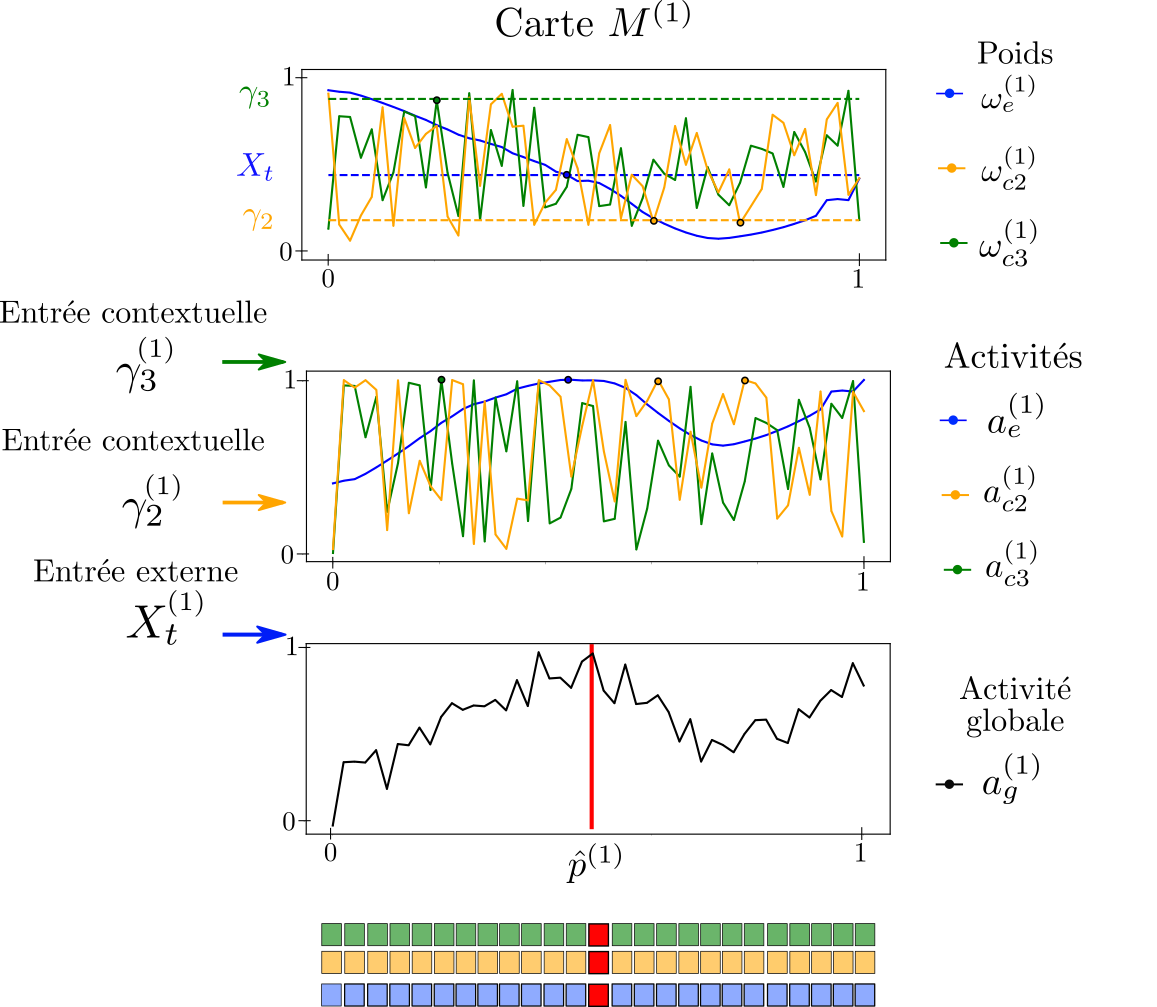
\includegraphics[width=0.8\textwidth]{activite_layers.pdf}
\caption{Calcul d'activité dans une SOM prenant plusieurs entrées au sein d'une architecture : une entrée externe et deux entrées contextuelles. L'indice $(1)$ permet de distinguer les objets relatif à cette carte. Les entrées externes sont $X\m{1}_t$. les deux entrées contextuelles sont $\inpc\m{1}_2$ et $\inpc\m{1}_3$. La carte possède trois couches de poids, permettant de calculer trois activités. L'activité globale prend en compte tout les couches d'activités afin de trouver un BMU commun pour toutes les couches de poids. Ce calcul favorise l'activité externe et est modulé par les activités contextuelles, ce qu'on observe sur la courbe du bas. Le maximum de l'activité globale est noté $\hat{p}$. A partir de l'activité globale, le BMU $\bmu\m{1}$ sera trouvé par le processus de relaxation décrit en partie suivante.}
\label{fig:activite}
\end{figure}

\subsection{Calcul du BMU par relaxation}

Contrairement à une carte simple, on ne peut pas calculer tous les BMUs de l'architecture d'un coup en prenant l'argmax de $a_g$ dans chaque carte.
A cause des influences mutuelles entre cartes, calculer le BMU d'une des cartes modifie les entrées des autres cartes de l'architecture, et donc leur BMU. 
On remplace donc l'étape de calcul d'argmax par un processus global à l'architecture de recherche de BMU. On cherche, dans chaque carte $i$, la position $\bmu\m{i}$ telle que $\forall i, a_g\m{i}(\bmu\m{i},\inpx\m{i},\bmu\m{i_0},\cdots,\bmu\m{i_k})$ soit maximale.
Cette recherche est réalisée par un processus dynamique que l'on appelera \emph{relaxation}, menant à un consensus entre cartes : on cherche un point, s'il en existe, où le BMU de chaque carte est au plus proche de son activité globale. On remplace l'étape de calcul d'argmax par le processus de relaxation.

Le processus de relaxation est une boucle imbriquée dans un pas d'apprentissage de l'architecture, indexée par $\tau$. Notons $\bmu\m{i}$ la position du BMU de la carte $i$, et $\mathbf{\bmu} = (\bmu\m{0}, \cdots , \bmu\m{n})$, avec $n$ le nombre de cartes de l'architecture.
Au début d'un pas d'apprentissage, chaque carte est nourrie avec une entrée externe, donc $\inpx\m{i}_t$ les activités externes $a_e\m{i}(\inpx\m{i}_t,p)$ de chaque carte peuvent être calculées.
La recherche du BMU suit le processus de relaxation suivant :
\begin{enumerate}
\item Dans chaque carte $i$, la position $\bmu\m{i}$ est initialisée à $\hat{p}\m{i}_0 = \argmax_{p\m{i}}(a_e\m{i}(\inpx\m{i}_t,p)$. Les entrées contextuelles de chaque carte peuvent ainsi être attribuées.
\item Tant que toutes les positions $\bmu\m{i}$ ne sont pas stables, 
	\begin{enumerate}
	\item Dans chaque carte $i$, calculer les activités contextuelles et globales, définissant ainsi $\hat{p}\m{i}_\tau = \argmax_{p\m{i}}(a_g\m{i}(p\m{i},\inpx\m{i}, \bmu\m{i_0}_\tau,\cdots,\bmu\m{i_k},_\tau)$, avec $i_0, \cdots, i_k$ les indices des cartes connectées à $i$ dans l'architecture.
	\item Déplacer $\bmu\m{i}$ vers $\hat{p}\m{i}$ : $\bmu\m{i}_{\tau +1} \leftarrow \bmu\m{i}_\tau \pm \Delta$ si $\lvert \bmu\m{i}- \hat{p}\m{i}\rvert \geq \Delta$, $\bmu^i \leftarrow p^{\star i}$ sinon
	\end{enumerate}
\item Le BMU de chaque carte est pris comme la valeur finale stable de ce processus dynamique. Cette valeur est utilisée pour les mise a jour des poids.
\end{enumerate}

Il peut arriver que les positions se stabilisent sur un cycle limite. Dans ce cas, on arrêtera la relaxation arbitrairement; ce phénomène étant ponctuel, il n'influence pas l'apprentissage. Les paramètres des cartes de l'architecture sont choisis pour éviter de telles situations.

\begin{figure}
\centering
\includegraphics[width=0.6\textwidth]{relaxation.pdf}
\label{fig:relax}
\caption{description d'une étape de la relaxation dans l'architecture, aboutissant à un consensus entre cartes. Au sein d'une même itération $t$, les position des BMU $\bmu$ sont légèrement déplacées jusqu'à ce que toutes les positions $\bmu$ des cartes de l'architecture soient stable. Ces positions maximisent collectivement les activités globales de chaque carte. }
\end{figure}

\begin{figure}
\centering
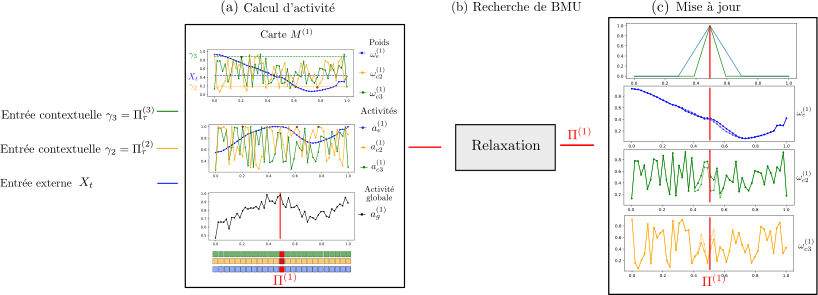
\includegraphics[width=\textwidth]{map_2layers.pdf}
\caption{Description d'une carte au sein d'une architecture CxSOM. La carte recoit deux connexions de cartes voisines, et possède donc deux couches contextuelles}
\label{fig:one_map}
\end{figure}

\subsection{Mise à jour des poids}

Les poids sont mis à jour par rapport à leurs entrées respectives suivant l'équation \ref{eq:update}. Le BMU d'une carte est ainsi commun à toutes les couches. Les rayons de voisinage $h_e$ et $h_c$ ont des valeurs différentes ; celles-ci seront détaillée en partie suivante. 
Il faut noter que les poids contextuels cartographient l'espace des positions d'une autre carte. Les positions des cartes sont donc associées par les poids contextuels.

\begin{figure}
\begin{minipage}[c]{0.5\textwidth}
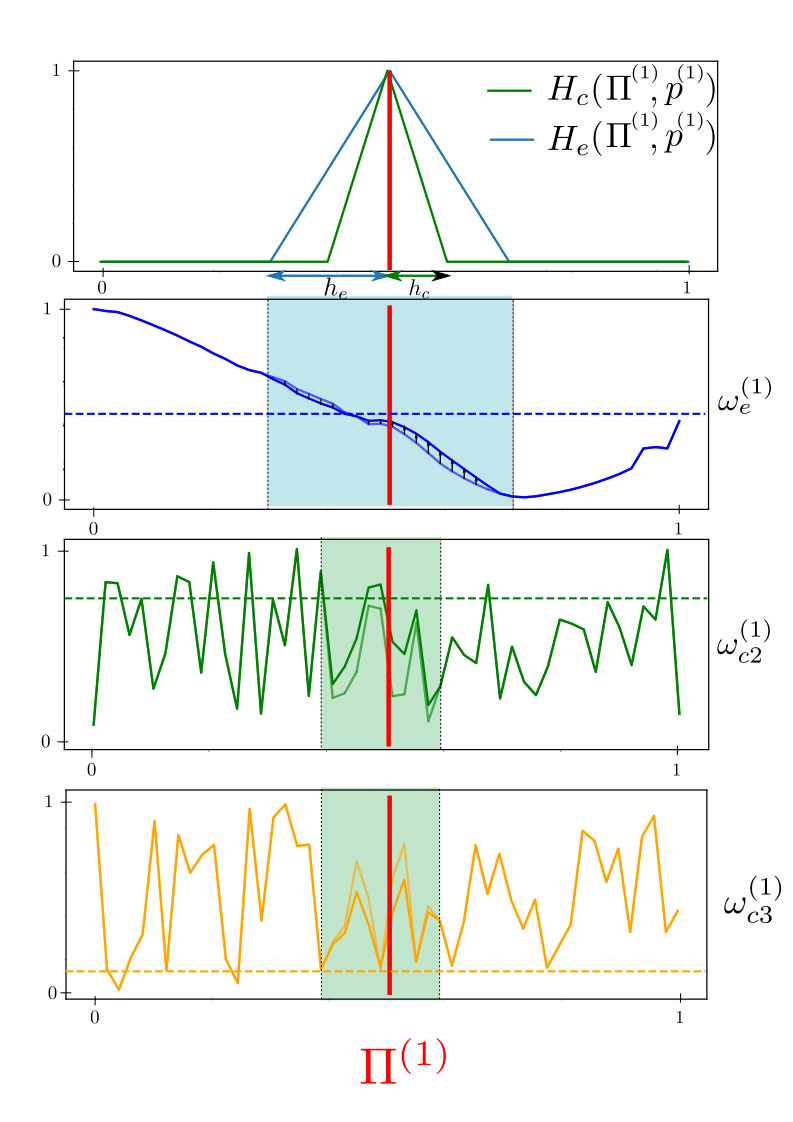
\includegraphics[width=\textwidth]{maj_layers.pdf}
\end{minipage}
\hfill
\begin{minipage}[c]{0.4\textwidth}
\caption{Mise à jour de chaque couche de poids indépendamment, relativement au BMU commun $\bmu\m{1}$. Le rayon de voisinage $h_e$ est utilisé pour mettre à jour les poids externes, le rayon $h_c$ pour mettre à jour les poids contextuels. On choisit $h_e > h_c$. Cette différence permet une différence d'échelle d'apprentissage entre couches de poids. Elle est détaillée en section suivante.}
\end{minipage}
\label{lig:maj}
\end{figure}
\subsection{Etape de test et prédiction d'entrée}

\subsection{Résumé : Algorithme général}

\begin{algorithm}\label{algo:relax}
\caption{Pas d'apprentissage $t$}
\SetAlgoLined
  \KwData{$\inpx\m{1}_t, ... , \inpx\m{K}_t$ tirés dans $\mathcal{D}\m{1} \times \cdots \times \mathcal{D}\m{n}$}
  $\tau \leftarrow 0$ \;
  \lForEach{Carte $i$}{$\bmu\m{i}_0 \leftarrow \argmax_{p\m{i}} a\ext(\inpx\m{i}_t,p\m{i})$}
  \While {$\mathbf{\bmu}_\tau \neq \mathbf{ \bmu}_{\tau-1}$ et $\tau < N_{max}$}{
  \ForEach{Carte $i$}{
  $\inpc\m{i}_1,...\inpc\m{i}_k \leftarrow \bmu\m{i_0}_\tau, \cdots, \bmu\m{i_k}_\tau$, $i_0, \cdots i_k$ indices des cartes connectées à $i$ dans l'architecture \;
	Calcul de $a_{c1}\m{i}(\inpc_1,p\m{i}), \cdots, a_{ck}\m{i}(\inpc_k,p\m{i})$ \;
  	Calcul de $a_g\m{i}(\inpx\m{i}, \bmu\m{i_0}_\tau, \cdots, \bmu\m{i_k}_\tau)$ (equation~\ref{eq:global_act}) \;
  $\hat{p}\m{i}_\tau = \argmax_{p\m{i}} a_g\m{i}(\inpx\m{i}, \bmu\m{i_0}_\tau, \cdots, \bmu\m{i_k}_\tau)$ \;
  Déplacement de $\bmu\m{i}_\tau$ vers $\hat{p}\m{i}$ d'un pas $\Delta$:
  $\bmu\m{i}_{\tau+1} \leftarrow \bmu\m{i}_\tau + min(\Delta, \lvert \hat{p}\m{i} - \bmu\m{i} \rvert) \times \sign(\hat{p}\m{i} - \bmu\m{i})$ \;
  }
  $\tau \leftarrow \tau + 1$ \;
  }
  $\bmu\m{1}, \cdots, \bmu\m{n} \leftarrow \hat{p}\m{1}_\tau, \cdots , \hat{p}\m{n}_\tau$ \;
  \ForEach{Carte $i$}{
  $\w\ext\m{i}(p) \leftarrow \w\ext\m{i}(p) + H\ext(\bmu\m{i}, p)(\w\ext\m{i}(p) - \inpx\m{i})$ \;
  \lForEach{$k$}{$\w_{ck}\m{i}(p) \leftarrow \w_{ck}\m{i}(p) + H\cont(\bmu\m{i},p)(\w_{ck}\m{i}(p) - \inpc\m{i})$}
  }
 \end{algorithm}
 
 \begin{algorithm}
\caption{Etape de test}
\SetAlgoLined

 \end{algorithm}
 
  \begin{algorithm}
\caption{Etape de Prédiction}
\SetAlgoLined
\KwData{$m$, indice de la carte servant à faire de la prédiction}

 \end{algorithm}

 

\section{Choix des paramètres}

\subsection{Paramètrage d'une carte}
On retrouve les mêmes paramètres dans CxSOM que sur une carte classique: taille de la carte, topologie et dimensions. 
Contrairement à une carte simple, on a maintenant un jeu de paramètre d'apprentissage par couche de poids d'une carte : pour chaque couche de poids $\w_e$ et $\w_{ck}$, on peut faire varier le taux d'apprentissage $\alpha$ et le rayon de voisinage $h_e$ ou $h_c$.
On choisit de prendre un taux d'apprentissage $\alpha$ commun à toutes les couches dans un souci de simplicité. $\alpha$ restera constant au cours de l'apprentissage, contrairement à une carte classique dans laquelle $\alpha$ décroît.
On choisit également de prendre des valeurs $h_{ck}$ communes à toutes les couches de poids contextuelles. Ainsi, on apporte une symétrie dans les connexions: les carte réagissent de la même façon aux autres cartes.
Par contre, on choisit de prendre le rayon externe $h_e$ très supérieur au rayon contextuel. Ce choix de paramètres apporte deux échelles de vitesse dans l'apprentissage, sans avoir à modifier les paramètres au cours du dépliement. Les poids externes se déplient alors très rapidement sur les données, quand les poids contextuels se déplacent très peu au début. Lorsque les poids externes sont organisés, l'apprentissage n'influence plus que les poids contextuels et ces derniers se déplient. 


\subsection{Paramètres de l'architecture}


\chapter{Méthodes de représentation et d'analyse de l'architecture CxSOM}
\graphicspath{{03-Representation/}}
\minitoc

\section{Introduction}
Dans le chapitre précédent, nous avons proposé l'algorithme CxSOM, permettant de construire des architectures non-hiérarchiques de cartes auto-organisatrices. 



Dans des architectures non-hiérarchiques, plusieurs cartes sont connectées et effectuent chacune une tâche d'apprentissage sur leur espace d'entrée externe, tout en prenant comme entrée secondaire les positions des \emph{Best Matching Unit} d'autres cartes. La particularité du modèle CxSOM est d'introduire des rétroactions entre cartes: l'architecture n'est pas un empilement de cartes qui apprennent tour à tour leurs entrées. 

Le but de ce modèle est de pouvoir construire des architectures assemblant un grand nombre de cartes; nous nous concentrons dans cette thèse sur des petites architectures de deux et trois cartes afin de comprendre les comportements qui émergent d'un tel système.

Nus étudions ces architectures sur une tâche particulière de mémoire associative. C'est-à-dire, parallèlement à l'objectif d'une SOM, qui consiste à effectuer de la quantification vectorielle sur un espace d'entrée, l'objectif d'une architecture de SOMs est de faire de la quantification vectorielle sur plusieurs espaces d'entrées et d'apprendre les relations existant entre ces entrées. 
Le but de cette thèse est d'analyser dans quelle mesure, et de quelle façon un tel apprentissage se déroule dans l'architecture de cartes construite avec CxSOM.

Au cours de cette thèse, nous cherchons à comprendre comment sont apprises les entrées et les relations entre les entrées au sein de l'architecture. La compréhension du comportement de blocs de quelques cartes posera en effet des bases pour la construction d'architectures plus grandes.
Ce système de cartes est un système complexe, même dans une architecture de quelques cartes. Nous voulons particulièrement poser un formalisme clair sur des architectures de quelques cartes pour permettre l'adaptation de CxSOM à plus grande échelle, mais nous ne cherchons pas à résoudre les équations d'évolution.
Cette thèse s'inscrit dans une démarche complètement expérimentale: nous observons l'organisation d'architectures de cartes sur différents espaces d'entrées, différents configurations, différents paramètres et pour comprendre leur comportement. 

L'évaluation de l'organisation d'une SOM classique est directe et très visuelle, cependant nous avons besoin de méthodes pour analyser l'organisation de ces cartes sur plusieurs entrées et plusieurs cartes. Nous posons dans ce chapitre la méthode expérimentale que nous utiliserons dans toutes les expériences présentées dans ce manuscrit. 
Le but de ce chapitre est de comprendre la démarche, comprendre les représentations et quels comportements sont observés d'après chaque représentation proposés. Nous voulons notamment répondre la question suivante: qu'est ce que signifie "les cartes ont appris des relations entre les entrées", et qu'est ce qu'une carte "bien organisée" dans le cas d'utilisation de CxSOM ?
Nous présenterons des représentations adaptées à cette méthode expérimentale et le formalisme utilisé. Le but de ce chapitre est de comprendre la démarche, comprendre les représentations et quels comportements sont observés d'après chaque représentation proposés. Nous voulons notamment répondre la question suivante: qu'est ce que signifie "les cartes ont appris des relations entre les entrées", et qu'est ce qu'une carte "bien organisée" dans le cas d'utilisation de CxSOM ?
Nous introduirons enfin un indicateur caractérisant l'apprentissage de ces relations entre entrées, basé sur l'information mutuelle.
Toutes ces représentations serons illustrées sur une architecture de deux cartes.

\subsection{Présentation de l'expérience d'illustration}

La méthode expérimentale sera présentée dans toute ce chapitre sur l'exemple très simple d'une architecture de deux cartes. L'architecture est illustrée à droite en figure~\ref{fig:exp}: elle est composée de deux cartes en une dimension. Chaque carte prend une entrée externe. Il s'agit de $\inpx\m{1}=x$ et $\inpx\m{2}=y$, les coordonnées de points 2D sur un cercle. Ces deux modalités sont dépendantes: pour une valeur de $x$, seule deux valeurs sont possible pour $y$, et symétriquement. Les entrées sont représentées sur le schéma de gauche, figure~\ref{fig:exp}.
Ces entrées externes sont normalisées entre 0 et 1. Les deux cartes sont des lignes 1D de 500 n\oe{}uds. Les rayons de voisinage sont $h_e = 0.2$ et $h_c = 0.02$.
Chacune des deux cartes est également connectée à sa voisine, c'est à dire, la carte $M\m{1}$ prend en entrée contextuelle la position du BMU de $M\m{2}$, et inversement.
%es données relatives à cette expérience et le code permettant de faire les tracés sont fournies sur git.
Afin de comprendre les tracés que nous présenterons, nous utiliserons deux cartes de Kohonen classiques en tant que témoin.
Une carte prend en entrée les valeurs $x$, et la deuxième les valeurs $y$, mais ces cartes ne sont pas connectées entre elles. Les paramètres de ces cartes sont les mêmes que les cartes de CxSOM: 500 n\oe{}uds et $h_e = 0.2$.

\begin{figure}
\begin{minipage}{0.4\textwidth}
\centering
\includegraphics[width=0.8\textwidth]{2som_inp_noinformation}
\end{minipage}
\begin{minipage}{0.6\textwidth}
\includegraphics[width=\textwidth]{2som_archi}
\end{minipage}
\caption{Disposition des entrée, sous forme de cercle, à gauche, et architecture de deux cartes en une dimension étudiée et représentée dans ce chapitre.\label{fig:exp}}
\end{figure}

\subsection{Représentations et indicateurs classique des cartes de Kohonen}

Les cartes de Kohonen sont particulièrement associées à une facilité de représentation et de visualisation. Leur nombre réduit de prototypes et leur aspect topologique permet d'en tracer une représentation visuelle interprétable.
La manière la plus couramment utilisée de représenter une carte de Kohonen est de tracer les poids de ses prototypes, disposés dans le graphe (ligne ou grille) qu'est la carte. En fonction des dimensions des entrées, cette représentation prennent plusieurs formes. Deux exemples courants de représentation sont les suivants: 
\begin{itemize}
\item Le graphe qu'est la carte de Kohonen est représenté dans l'espace de ses positions (la grille d'indices $(i,j)$, ou une ligne indexée par $i$. Sur chaque noeud est tracé le poids correspondant. C'est le cas sur l'exemple de gauche en figure~\ref{fig:representation} dans lequel les poids des prototypes, qui sont des imagettes, sont affichés en chaque point de la grille. 
%Si la dimension d'un poids est trop grande pour être représentée graphiquement, il est également courant d'étiquetter chaque prototype et d'afficher ces étiquettes sur les n\oe{}uds de la carte, en tant que représentation.
\item Lorsque les données traitées sont des points deux ou trois dimensions, les poids des prototypes peuvent être directement tracés dans l'espace $\mathbb{R}^2$ ou $\mathbb{R}^3$. Ces poids sont alors reliés en fonction des positions des n\oe{}uds dans la carte, montrant ainsi la déformation de la carte dans l'espace d'entrée, c'est le cas sur l'exemple de droite en figure~\ref{fig:representation}.
\end{itemize}

\begin{figure}
\begin{minipage}{0.5\textwidth}
\centering
\includegraphics[width=0.5\textwidth]{digits.jpg}
\end{minipage}
\begin{minipage}{0.5\textwidth}
\centering
\includegraphics[width=0.5\textwidth]{points.png}
\end{minipage}
\caption{Représentations possible des poids d'une carte de Kohonen classiques, dans le cas d'entrées sous forme d'imagettes ou de points en deux dimensions.\label{fig:representation}}
\end{figure}

\subsection{Limites de la représentation classique pour CxSOM}

Utilisons les représentations classiques mentionnées ci-dessus pour tracer les poids de chacun des cartes d'une architecture CxSOM. Les poids sont tracés à la fin de l'apprentissage. On définit la fin de l'apprentissage lorsque les poids on convergé vers une organisation stable selon les itérations $t$.
La figure~\ref{fig:weights} présente le tracé des poids des deux cartes de l'exemple.
La courbe orange correspond aux poids externes, se dépliant sur chaque coordonnée $x$ et $y$ des points du cercle, appartenant chacune à $[0,1]$. Ce tracé permet d'observer que les poids externes couvrent l'intervalle $[0,1]$, et sont organisés de façon monotone, comme on l'attend dans une carte simple. Les poids contextuels, en bleu, ne présentent pas cette organisation monotone, mais présentent une continuité: deux prototypes proches ont des poids proches. Le tracé nous informe donc sur le caractère continu de l'organisation de chacune de couches de poids. 

Notons que nous ne pouvons pas en tirer plus de conclusion: la représentation des poids de la figure~\ref{fig:weights} ne différencie pas les n\oe{}uds qui seront effectivement BMUs, des n\oe{}uds \emph{morts}. Ces n\oe{}uds morts ont bien un poids, mais ne seront jamais BMUs. Dans une carte de Kohonen classique, ces n\oe{}uds correspondent à des transitions, liant deux zones denses de l'espace d'entrée séparée par une zone sans points.
Par ailleurs, cette représentation concerne une seule carte. Nous ne pourrons pas tirer des informations sur l'influence des connexions entre cartes à partir de ces représentations.

Il est donc nécessaire de trouver un moyen de représenter l'architecture comme un tout. Nous devons définir une représentation qui montre comment l'architecture de cartes est capable d'apprendre les relations entre les entrées multimodales.

Lorsque la dimension des entrées ou le nombre de cartes sont élevés, une représentation graphique ne suffit plus: il y a trop d'éléments à représenter. Cette difficulté de représentation soulève la nécessité de définir des valeurs indicatrices du fonctionnement de la carte qui soient calculables en grande dimension.

% Enfin, la représentation visuelle d'une cartes d'une architecture est limitée par la dimension des entrées et la dimension des cartes. Dans l'exemple, les entrées et les cartes sont en une dimension, représenter leurs poids est donc réalisable.
% En plus grande dimension, il sera nécessaire d'utiliser une représentation telle que celle décrite en figure~\ref{fig:representation}. Le nombre de connexions contextuelles limitera alors également la lecture d'un tracé. Cette difficulté de représentation soulève la nécessité de définir des valeurs indicatrices du fonctionnement de la carte, calculables en grande dimension.

\begin{figure}
\centering
\includegraphics[width=0.9\textwidth]{weights_cercle1.pdf}

\caption{Représentation des valeurs des poids d'une carte au sein de CxSOM après apprentissage. La seule représentation de ces poids ne suffit pas à savoir comment la carte se comporte.\label{fig:weights}}
\end{figure}

Ce chapitre questionne donc la façon de représenter une carte au sein d'une architecture. Nous présenterons en premier lieu le formalisme décrivant les cartes et leurs entrées multimodales associées ainsi que la méthode expérimentale que nous utiliserons pour toutes les expériences présentées dans cette thèse. A partir de ce formalisme, nous proposerons plusieurs représentations et indicateurs permettant de comprendre et représenter ce que calcule une architecture CxSOM sur les données d'entrées.

\section{Formalisation par variables aléatoires}

Nous introduisons dans cette section un formalisme traitant les éléments des cartes et les entrées en tant que variables aléatoires. 
Ce formalisme a l'avantage de à la fois clarifier les représentations et de permettre le développement d'indicateurs statistiques sur les cartes.

\subsection{Représentation des entrées}

Nous nous placons dans une tâche de mémoire associative. Nous considérons plusieurs espaces d'entrée $\mathcal{D\m{1}},\cdots,\mathcal{D\m{n}}$ dont seront tirées les entrées présentées au cartes. Chaque espace est une modalité.
Les observations multimodales que l'on cherche à apprendre par l'architecture de cartes sont notées $(\inpx\m{i} \in \mathcal{D}\m{i}, i = 1 \cdots n)$. Les $\inpx\m{i}$ sont modélisées comme des variables aléatoires. Chaque variable aléatoire possède ainsi une distribution $p\m{i}(\inpx\m{i})$ sur $\mathcal{D}\m{i}$.
Nous notons $\mathbf{\inpx} = (\inpx\m{1}, \cdots, \inpx\m{n})$ la variable aléatoire jointe. Cette variable appartient à l'espace $\mathcal{D}\m{1} \times \cdots \times \mathcal{D}\m{n}$. Elle a une distribution jointe. La distribution de probabilité de chaque modalité $\inpx\m{i}$ sur son espace $\mathcal{D}\m{i}$ est alors une distribution marginale de $\mathbf{X}$.


A chaque pas de temps, un vecteur $\mathbf{\inpx} = (\inpx\m{0}_t, \cdots , \inpx\m{N}_t)$ est présenté à l'architecture: il s'agit d'une réalisation de la variable jointe $\mathbf{\inpx}$. On s'intéresse à l'apprentissage de relations entre entrées: les variables $\inpx\m{i}$ ne sont pas des variables indépendantes.

En pratique, ces variables sont des observations, issues par exemple de capteurs d'un robot. Ces observations sont issues d'un d'environnement général qui est modélisable. 
Nous introduisons la notion de \emph{modèle d'entrées}, se rapportant à cette dépendance entre variables.
Le modèle d'entrée fait référence au modèle d'environnement permettant de générer les entrées multimodales fournies en entrées. Dans l'exemple d'illustration, les modalités sont les abscisses $\inpx\m{1} = x$ et les ordonnées $\inpx\m{2} = y$; le modèle d'entrées correspond à l'équation du cercle.

Le but de l'apprentissage non supervisé par des cartes de Kohonen est d'apprendre une représentation discrète de l'espace d'entrée.
Avec CxSOM, nous chercherons à la fois à apprendre un représentation discrète des espaces d'entrée, mais aussi d'apprendre une représentation du modèle d'entrées.

Les tracés et indicateurs que nous développerons dans cette section ont pour but de mesurer comment ce modèle est appris par l'architecture. 

\subsection{Démarche expérimentale}

Afin d'étudier le comportement de la carte à un instant $t$ de l'apprentissage, nous réalisons une phase de test.
Lors de la phase de test, des entrées sont présentées à la carte, mais seul le processus de recherche de la best matching unit est réalisé. Les poids des cartes ne sont donc pas mis à jour. Ce processus de test génère un ensemble de réponses de la carte aux entrées présentées. Le processus d'apprentissage et de tests est décrit en figure~\ref{fig:flowchart}.
Les entrées utilisées lors du test sont un ensemble de réalisations de la variable aléatoire $(\inpx\m{1}, \cdots, \inpx\m{n})$.
Définissons aussi des variables aléatoires pour chaque élément des cartes. Ces éléments sont les positions des BMUs, représentées par des variables aléatoires $\bmu\m{1}$ et $\bmu\m{2}$ et leurs poids $\w\ext\m{1}(\bmu\m{1})$ et  $\w\ext\m{2}(\bmu\m{2})$. Entre deux itérations de test, la valeur de ces éléments ne dépend que de l'entrée, car les poids ne sont pas mis à jour. 
Une phase de test est donc un ensemble de réalisations d'une variable aléatoire jointe : 
$$(\inpx\m{0}, \cdots, \inpx\m{N}, \bmu\m{0}, \cdots, \bmu\m{N}, \w_e\m{0}(\bmu\m{0}), \cdots, \w_e\m{N}(\bmu\m{N}))$$
Les composantes de cette variable jointe ne sont pas indépendantes. Les représentations et indicateurs présentés ensuite chercheront à détecter et comprendre au mieux leurs dépendances statistiques.
Les échantillons de test utilisés dans cette partie contiennent 1000 éléments.
Le formalisme par variable aléatoires permet d'utiliser des outils et métriques issus de la théorie de l'information pour qualifier l'organisation des cartes au sein de l'architecture.

\begin{figure}
\centering
\includegraphics[width=0.85\textwidth]{tests_2maps.pdf}
\caption{Schéma descriptif des tests}
\label{fig:flowchart}
\end{figure}


\section{Tracés}

A partir des échantillons de tests, nous proposons dans cette section les représentations graphiques que nous utiliserons et leur intérêt.
Il s'agit de tracer les dépendances entre les variables $$(\inpx\m{0}, \cdots, \inpx\m{N}, \bmu\m{0}, \cdots, \bmu\m{N}, \w_e\m{0}(\bmu\m{0}), \cdots, \w_e\m{N}(\bmu\m{N}))$$, dont les valeurs sont obtenues lors du test.
% Ces points se superposent à la courbe de poids, mais certaines unités ne seront pas représentées: on les appelles \emph{unités mortes}. La position de la best matching unit $\bmu$ étant la réponse de la carte à une entrée, il s'agit d'un tracé d'un élément de la carte en fonction de la réponse de celle-ci.

%\subsection{Représentation des entrées par rapport au BMU}
\subsection{Cartographie des entrées}

En première représentation, nous tracerons les valeurs de l' entrée $\inpx\m{i}$ d'une carte par rapport à la position du BMU $\bmu\m{i}$.
Cette représentation permet d'analyser la quantification des entrées par la carte.
Ces tracés sont réalisables pour des cartes une et deux dimensions, pour des entrées quelconques, que ce soient des réels ou des entrées de plus grande dimension comme des images.
On s'attend à ce que les points soient proches de la courbe des poids externes de la carte $M\m{i}$.
Ce tracé fait apparaître les zones qui ne sont jamais best matching unit.

Sur le même graphique, nous affichons non seulement les poids $(\bmu\m{i},\inpx\m{i})$ mais également les entrées des autres cartes, également en fonction de $\bmu\m{i}$.
En figure~\ref{fig:inputs}, nous avons ainsi tracé les points $(\bmu\m{1},\inpx\m{1})$ et $(\bmu\m{1},\inpx\m{2})$ issus de l'expérience sur les deux cartes.

Cette façon de représenter les réponse d'une carte s'inspire la façon de cartographier les aires du cortex cérébral en biologie.
Dans ces représentations, la valeur d'entrée faisant réagir un neurone est indiquée en fonction de sa position dans le cortex.
Par exemple, une carte corticale est tracée pour l'aire visuelle primaire du cortex cérébrale, l'aire v1, en figure~\ref{fig:v1_repr}.

\begin{figure}
    \centering
    \includegraphics[width=0.7\textwidth]{v1.jpg}
    \caption{Carte corticale de l'aire cérébrale visuelle V1. Pour tracer cette représentation, un ensemble de traits de différentes orientation sont présentés en stimuli visuels au sujet, indiqués en bas de l'image. Le neurone réagissant à une entrée d'orientation particulière est coloré sur la carte de la couleur correspondante à l'entrée. Cette méthode permet de tracer des \emph{cartes corticales} d'une aire cérébrale. Source:~\cite{Bosking1997OrientationSA}.\label{fig:v1_repr}}
\end{figure}

\begin{itemize}
    \item But: observer si les entrées externes sont proches de la courbe de poids externes
    \item Différencier les unités mortes des unités étant effectivement BMU
    \item Mettre en relation les entrées $\inpx\m{1}$ et les entrées $\inpx\m{2}$ sur un même schéma.
\end{itemize}

% On s'attend à ce que les entrées externes soient proche de la courbe de poids externes. Cela indiquera que le poids externe $\w\ext\m{1}(\bmu\m{1})$ est une approximation de $\inpx\m{1}$ et qu'une carte réalise de la quantification vectorielle sur ses entrées externes, malgré les connexions à l'autre carte. On attend également que la présence de la connexion avec $M\m{2}$, par l'entrée contextuelle, influence l'organisation de $M\m{1}$; et, si possible, qu'un modèle de connexions d'entrée est appris.

% Ce tracé est présenté en figure~\ref{fig:inputs}. On représente la valeur des entrées $\inpx\m{1} = x$, en orange, et $\inpx\m{2}=y$, en bleu, par rapport à la position du BMU dans la carte $M\m{1}$, $\bmu\m{1}$. Ce tracé sur l'architecture de deux cartes (c) est comparé à ce qu'on obtient si les valeurs de $x$ étaient présentés à une carte classique (b). Les poids externes sont représentés en bleu, les poids contextuels en orange. Deux échantillons du schéma des entrées (a) sont mis en valeur, en bleu et rouge. Ces deux points ont la même valeur pour $x$, mais deux valeurs différentes pour $y$. Ces échantillons sont reportés en couleur sur les deux tracés (b) et (c).


% Analysons d'abord la forme des poids contextuels de $M\m{1}$, que nous avions tracés en figure~\ref{fig:weights} sans les commenter. Les poids externes, en orange, présentent une disposition similaire à ceux observés dans la carte classique (b). Les poids contextuels, en bleu, présentent une forme de vagues, avec 7 valeurs de maximum allant de 0.5 à 1, et 6 minimum allant de 0.5 à 0.1. Ces maximum et minimum sont répartis en zones de taille équivalente sur la carte. 

% Lorsqu'on s'intéresse au tracés des échantillons, on remarque d'abord que les positions dans la carte $M\m{1}$ se répartissent en zones étant BMUs et zones mortes, dans lesquelles aucune entrée n'a gagné. C'est une première différence avec la carte indépendante, pour laquelle toutes les positions gagneront pour des entrées. Les zones dans lesquelles il y a des BMUs correspondent aux extremum des poids contextuels et leurs alentours. C'est un phénomène inhabituel pour une carte de Kohonen. Les entrées $\inpx\m{1}$, dans la carte classique (b), correspondent à la courbe de poids externe: la valeur du poids du gagnant est toujours très proche de la valeur de l'entrée. Dans la carte $M\m{1}$, les entrées externes $\inpx\m{1}$ orange sont proches de la courbe de poids externes, mais avec plus d'erreur de quantification.
% Les deux points rouge et bleu ayant la même valeur de $x$ ont un BMU différent dans la carte $M\m{1}$, alors que ces deux échantillons ont le même BMU dans la carte apprenant indépendamment sur les valeurs de $x$. Ainsi, la carte connectée au sein de CxSOM différencie les échantillons en fonction de non seulement leur entrée externe, mais aussi de l'entrée de l'autre carte de l'architecture. La plage de valeurs des $\inpx\m{1}$ gagnant dans un des zones recoupe les plages de valeurs gagnant dans les zones situées à gauche et à droite. Par exemple, la zone dans laquelle l'échantillon rouge gagne, autour de $\bmu\m{1} = 0.25$. La partie des entrées située en dessous de la courbe de poids externe recoupe les valeurs d'entrées gagnant dans la zone précédente; la partie située au dessous de la courbe de poids externe recoupe des valeurs gagnant dans la partie suivante. Pour une entrée externe, le choix de la zone de BMU dans laquelle elle gagnera dépend alors de l'entrée contextuelle. 


% Dans la carte $M\m{1}$, une unité se spécialise donc par rapport aux deux entrées et non pas une seule comme dans la carte indépendante: les entrées externes et l'entrée contextuelles. C'est bien ce à quoi on s'attendait en ayant deux couches de poids. Ce qui est intéressant est que cette différenciation est réalisée par la répartition des unités en un nombre fini de zones distinctes. Dans chaque zone, les unités sont BMUs pour un segment de valeurs d'entrée externe et contextuelles. Au sein d'une zone, la répartition des entrées externe selon le BMUs est ordonnée, comme ce serait le cas dans une carte auto-organisatrice classique. Le comportement de la carte au sein d'une zone reste donc similaire à celui d'une carte classique.

% Deux zones adjacentes correspondent par ailleurs à des segments de valeur d'entrée en partie superposés, et des segments de valeurs d'entrées contextuelles différentes. Il s'agit d'une deuxième échelle d'organisation, qui garde également l'aspect ordonné d'une carte classique. Ces zones sont créées par auto-organisation; aucun paramètre de la carte n'a été modifié pendant l'apprentissage pour former ces zones, et le nombre d'unités allouées par auto-organisation dans chaque zone est à peu près égal. La carte agit un peu comme une base de données structurée avec des indices primaires et des indices secondaires pour chaque neurone, l'indice primaire étant la zone de la carte, et l'indice secondaire la position dans cette zone.

\begin{figure}
\begin{minipage}{0.27\textwidth}
\includegraphics[width=\textwidth]{2som_inp.pdf}
\end{minipage}
\begin{minipage}{0.34\textwidth}
\includegraphics[width=\textwidth]{weights_2som_unco.pdf}
\end{minipage}
\begin{minipage}{0.38\textwidth}

\includegraphics[width=\textwidth]{weights_2som.pdf}
\end{minipage}

\caption{Représentation des entrées $X$,$Y$ d'une architecture de deux cartes relativement au BMU de la carte $X$ après apprentissage. Ces tracés mettent en valeur l'organisation des cartes, différentes dans le cas ou les cartes apprennent indépendemment leurs entrées~(b) ou sont connectées~(c). Les entrées correspondantes sont en figure~(a). Les points bleu et rouge reportés sur les tracés correspondent au même échantillon de test.\label{fig:inputs}}
\end{figure}

\subsection{Réduction de dimension des entrées}

Lorsque la dimension totale des entrées dépasse trois, l'interprétation visuelle de toutes les entrées sur le tracé précédent n'est plus possible. Dans ce cas, la méthode classique de représentation passe par une réduction de dimension des entrées. Ces méthodes de réduction de dimension, telles que T-SNE~\cite{Maaten2008VisualizingDU} ou  l'analyse en composantes principales sont largement utilisées dans les applications de l'apprentissage automatique, la dimension des éléments qu'on cherche à observer étant rarement faible.
A partir des données d'entrée en grande dimension, la réduction de dimension cherche à associer à chaque échantillon une valeur de plus faible dimension, en l'occurence deux ou trois, pour qu'elle puisse être représentée sur un graphique. Cette valeur de dimension plus faible doit être une "bonne" représentation des données originale. La qualité de cette représentation dépend de l'algorithme utilisé. Ainsi, T-SNE conserve la proximité entre les points, la PCA conserve les axes sur lesquels la covariance est maximale.
Notons que la réduction de dimension, dans la plupart des cas, perd de l'information. Cette perte d'information doit être prise en compte lors de l'analyse des données.

Nous nous placerons dans des cas particulier de réduction de dimension sans perte d'information.
Dans notre cas particulier, les entrées sont générées par un modèle géométrique. Dans ce cas, on va pouvoir effectuer une réduction de dimension en faisant une paramétrisation géométrique du modèle générant les entrées.
Nous définissons une variable supplémentaire $U$, de dimension inférieure ou égale à la somme des dimensions des entrées.
Elle choisie de façon à ce que chaque variable $\inpx\m{i}$ soit une fonction de la variable aléatoire $U$, et uniquement de cette variable.

\begin{equation}
\forall i, \inpx\m{i} = f\m{i}(U)
\label{eq:U}
\end{equation}

Pour que la variable $U$ conserve toute l'information sur le modèle, la fonction $(f\m{1}, \cdots, f\m{N})$ : $(\inpx\m{1}, \cdots \inpx\m{N})\rightarrow U$ doit être une bijection. Toute valeur jointe d'entrée correspond à un seul $U$, toute valeur de $U$ renvoie à une seule valeur d'entrée jointe. 
Cet aspect est un cas particulier par rapport aux méthodes de réduction de dimension classique, car il n'y a pas de perte d'information.
Dans le cas d'exemple, $\mathbf{X} = (X,Y)$, les coordonnées cartésiennes des points du cercle est alors une vecteur aléatoire, dont les composantes sont les variables aléatoires $X,Y$. En définissant une variable $U$ à valeurs dans $[0,1]$, chaque point du du cercle peut maintenant s'écrire, selon l'équation paramétrique du cercle:
\begin{equation}
 \begin{cases}
     X = r  \cos(2\pi U)\\
     Y = r \sin(2 \pi U)
    \end{cases}\,.
\end{equation}

$U$ représente ici l'angle du point sur le cercle (à un facteur $2\Pi$ près). $U$ est une variable cachée qui réduit la dimension du modèle.  Les exemples donnés sont scalaires, mais cette représentation générale à n'importe quel dimension et nombre d'entrées.

Cette variable ajoute donc un attribut aux données échantillonnées durant une phase de test. Une phase de test donne donc un ensemble de valeurs de $U$, en plus des positions de BMUs $\bmu\m{i}$ et de leurs poids.

\begin{figure}
\centering
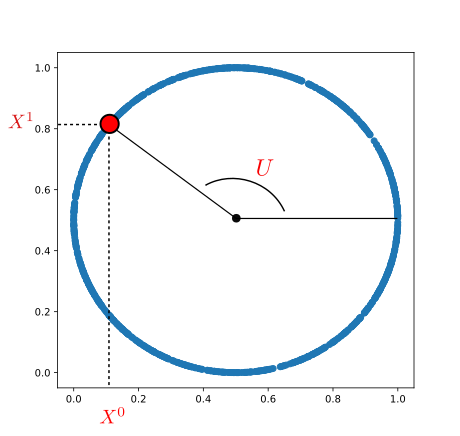
\includegraphics[width=0.6\textwidth]{cercle.pdf}
\caption{Représentation choisie pour le cercle. Le modèle auxquelles appartiennent les modalités $X^0$ et $X^1$ est représenté par la variable cachée $U$. \label{fig:U}}
\end{figure}

Nous tracerons les nuages de points $U$ en fonction de la position $\bmu$ du BMU d'une carte pour représenter comment la position du BMU traduit la relation entre les entrées. Dans le cas de l'expérience à deux cartes, $U$ est en une dimension, et le tracé est présenté en figure~\ref{fig:piu}. 

En figure~\ref{fig:piu}, nous tracons ainsi $U$ en fonction de $\bmu\m{1}$ et $U$ en fonction de $\bmu\m{2}$. Nous avons observé sur les tracés en figure~\ref{fig:inputs} que chaque carte allouent leurs unités en fonction des deux entrées. En tracant $U$ en fonction de la position du BMU, on retrouvera d'abord les zones de la cartes. 

% Le tracé en figure~\ref{fig:piu} montre $U$ comme une fonction de la position du BMU dans chaque carte, contrairement au cas ou les cartes ne sont pas connectées. 
% En effet, dans ce dernier cas, il y a plusieurs valeurs de $U$ pour un même $\bmu$, une valeur $x$ de $\inpx\m{1}$ correspondant à deux positions sur le cercle.
% L'organisation en zones rend une position $\bmu$ codant pour une seule valeur de $U$, c'est à dire une seule position d'échantillon sur le cercle. $U$ est alors une fonction de $\bmu$, ce qui est représenté en pointillé sur la figure~\ref{fig:piu}. Donc, chaque carte $M\m{1}$ et $M\m{2}$ code pour toute l'architecture, par les deux couches de poids, et non plus seulement son entrée.

% La forme générale du tracé de $U$ selon $\bmu\m{i}$ dans chaque carte est proche du tracé obtenu dans le cas des cartes indépendantes. Une carte de l'architecture se comporte donc comme une carte classique, dans laquelle les connexions contextuelles viennent moduler la réponse. La réponse d'une carte garde une continuité par rapport à $U$.
\begin{figure}
\centering
\includegraphics[width = 0.7\textwidth]{xu_yu_both.pdf}
\caption{Valeur de $U$ en fonction des valeurs du BMU $\bmu\m{i}$ dans chacune des cartes, pour des entrées prises sur le cercle. Sur la première ligne, nous tracons la réponse de chaque carte à son entrée dans le cas ou les cartes ne sont pas connectée. Sur la deuxième ligne, nous traçons la réponse de chaque carte lorsqu'elles ont appris de façon jointe au sein de CxSOM.
$U$ apparaît alors comme une fonction de la position du BMU $\bmu\m{i}$ dans chaque carte, contrairement au cas ou les cartes apprendraient indépendamment sur les mêmes entrées. Cette relation fonctionnelle est symbolisée par les pointillés sur les tracés du bas.}
\label{fig:piu}
\end{figure}

La représentation de $U$ selon la position du BMU d'une carte $\bmu\m{i}$ permet de représenter comment la carte $i$ a appris l'ensemble d'entrées $(\inpx\m{1},\inpx\m{2})$ et non seulement son entrée externe.

Ces tracés sont également faisables et ont un intérêt avec une méthode de réduction de dimension classique. 

\subsection{Représentation de l'erreur de quantification dans une carte}

Afin de mesurer la qualité de la quantification vectorielle au sein d'une carte dans CxSOM, nous tracerons, pour un échantillon test, le poids externe du BMU $\w_e(\bmu\m{i})$ en fonction de l'entrée présentée $\inpx\m{i}$. 
Si une carte a appris bonne représentation correcte de ses entrées externes, la forme de ce tracé doit être proche de l'identité. 

En figure~\ref{fig:erreur}, nous avons tracé le poids du BMU de chaque carte en fonction de l'entrée qui lui a été présentée, dans l'expérience à deux cartes. Ces tracés s'approchent de l'identité: la quantification des entrées est correctement réalisée. On observe une erreur plus grande que dans le cas d'une carte isolée qui aurait le même nombre de neurones, c'est à dire 500 ici. Dans ce dernier cas, les 500 neurones permettent aux poids de se disposer densément entre 0 et 1..

\begin{figure}
    \centering
    
\includegraphics[width=0.7\textwidth]{w_x.pdf}
    \caption{Poids du BMU dans chaque carte en fonction de l'entrée présentée. On s'attend à des tracés proches de l'identité, montrant que le poids du BMU d'une carte est une bonne représentation de l'entrée. Sur ce graphique, on se rapproche effectivement de la fonction identité, cependant, une faible erreur est observée. On observe également un découpage des poids en bandes.\label{fig:erreur}}
\end{figure}

\draft{\subsection{Dépliement d'une carte en plusieurs dimensions}

\subsubsection{Méthode}
Nous avons vu qu'analyser le comportement d'une carte en fonction de toutes les entrées est un moyen de mieux comprendre la représentation interne qu'a une architecture sur le modèle d'entrée.
Nous proposons ici une façon originale de représenter les poids d'une carte de Kohonen dans l'espace de toutes les entrées. Cette représentation est faisable lorsque la dimension totale des entrées est de deux ou trois. Nous utiliserons donc cette représentation seulement sur les données géométriques, afin de mieux comprendre l'organisation des cartes.

Cette représentation est crée à partir des échantillons de test. Il s'agit de tracer les poids externes des BMUs dans l'espace de toutes les entrées: $(\w_e(\bmu\m{1}),\cdots,\w_e(\bmu\m{k}))$ dans l'espace en $k$ dimensions correspondant - $k$ correspondant ici à 2 ou 3 dimensions. Les échantillons sont ensuites reliés suivant l'ordre des positions dans \emph{une des cartes}. On obtient ainsi le \emph{dépliement} d'une carte de l'architecture dans l'espace multimodal à plusieurs dimensions. 

\subsubsection{Résultats}

Un exemple de carte ainsi dépliée est présenté en figure~\ref{fig:distortion}.

\begin{figure}
\begin{minipage}{0.5\textwidth}
\centering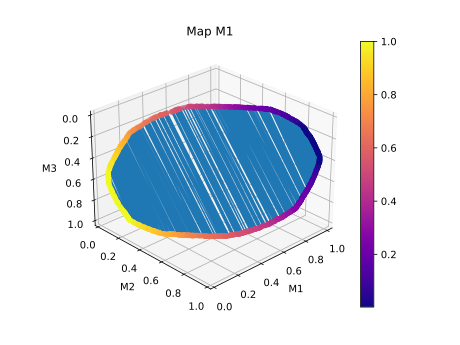
\includegraphics[width=0.8\textwidth]{unco3som}
\end{minipage}
\begin{minipage}{0.5\textwidth}
\centering\includegraphics[width=0.8\textwidth]{disto_Mx}
\end{minipage}
\caption{Représentation des poids finaux de trois cartes prenant en entrée les coordonnées des points d'un cercle: $x = \inpx\m{1}$,$y = \inpx\m{2}$ et $z=\inpx\m{3}$, reliés selon les positions de la carte $X$. A gauche, les cartes de l'architecture ont appris séparément sur les données. A droite, disposition lorsque les cartes ont été connectées au sein d'une architecture. Un échantillon de 1000 points a été utilisé pour les tracés.}
\label{fig:distortion}
\end{figure}

Ces figures sont équivalentes à tracer une carte dans l'espace de ses entrées: les poids des BMUs de l'échantillon sont les prototypes des cartes; seuls les poids des unités mortes ne sont pas représentés.
Cette représentation est limitée par la dimension des entrées, mais elle peut-être étendue: en plus grande dimension, il est possible de tracer le dépliement de la carte selon un sous-espace choisi de chacune des modalités, ou après réduction de dimension.
Par ailleurs, l'étude du comportement de cartes sur des données 3D s'inscrit dans la démarche de construction d'un modèle que nous suivons dans cette thèse. Leur visualisation est alors un élément clé dans la compréhension des comportements possibles de l'architecture. A partir de cette visualisation, on peut envisager de construire des indicateurs permettant l'analyse de l'architecture en dimension supérieure. 

Le second avantage de ces tracés est qu'il est possible de représenter graphiquement une carte qui ne prend pas d'entrée externe, ou de représenter une carte dans l'espace des poids d'autres cartes.
}

\section{Un indicateur de l'apprentissage du modèle par l'architecture}

L'étude de tout processus physique s'effectue par un ensemble signaux issus de capteurs. La théorie de l'information de Shannon \cite{Shannon1948AMT} apporte un modèle mathématique qui abstrait ces signaux et permet de les manipuler, les encoder, les décoder et quantifier l'apport ou perte d'information entre eux, en les utilisant en tant que distributions de probabilités.
Ce modèle mathématique puissant permet de s'abstraire de la nature des signaux pour s'intéresser à leurs relations. Comme son nom l'indique, la théorie de l'information s'appuie sur la notion fondamentale d'information portée par un symbole. Ensuite, cette information se décline en quantités qu'on calcule en fonction de ce qu'on veut mesurer: l'entropie d'une variable, comme l'information apportée par l'observation de la variable seule; l'entropie conditionnelle entre deux variables,l'information mutuelle entre deux variables ou un plus grand nombre. Ces mesures définissent une dépendance statistique générale, et ne dépendent pas du type de modèle ou de relation.

Nous investiguerons dans cette partie comment quantifier l'apprentissage de l'architecture de cartes par des outils d'information. Bien que cette théorie soit un outil mathématique puissant, il s'agit d'un modèle s'appuyant sur les probabilités. L'estimation à partir de données est donc un élément clé et parfois limitant lorsqu'on cherche à utiliser des valeurs telles que l'entropie pour quantifier l'information au sein d'un système. Nous définirons donc dans cette partie des quantités à mesurer dans l'architecture de cartes, et chercherons à l'estimer.

\subsection{Information mutuelle et entropie}

Les notions d'\emph{entropie} et les valeurs qui en sont dérivées, telle que l'\emph{information mutuelle} entre des distributions, sont des notions fondamentales de la théorie de l'information de Shannon. Ces quantités donnent des informations concernant la distribution d'une variable aléatoire.
Les formules indiquées dans ce paragraphe concernent des variables aléatoire discrètes. 
L'entropie de Shannon d'une variable aléatoire $X$ à valeurs discrètes dans un ensemble $E_X$, de distribution $p(X)$, est notée $H(X)$ et définie par la formule : 
\begin{equation}
H(X) = - \sum_{x \in E_X}{p(x)\textrm{log}(p(x))}
\end{equation}

Elle se mesure en $bit/symbole$ lorsque le logarithme est en base 2, ce qui est généralement utilisé. 
L'entropie est une mesure de la quantité d'incertitude, ou de surprise, sur la valeur de la variable aléatoire $X$. Si la la distribution de probabilité de $X$ est concentrée autour d'un point, l'entropie est faible : lors d'une réalisation de $X$, l'observateur est \emph{plutôt certain} du résultat. En revanche, l'entropie est maximale lorsque lorsque $X$ suit une distribution de probabilité uniforme.
L'entropie s'interpète également comme la quantité moyenne d'information à fournir, en bits, pour coder la valeur que prend la variable $X$.
De la même manière, on peut définir l'entropie conjointe de deux variables, qui est l'entropie de leur distribution jointe, et l'entropie conditionnelle, qui est l'entropie de leurs distributions conditionnelles.

Outre les entropies jointes et conditionnelles, les relations statistques entre deux variables aléatoires $X,Y \in E_X,E_Y$ peuvent être mesurées par \emph{l'information mutuelle}. Elle se définit formellement par : 
\begin{equation}
 I(X,Y) = \sum_{x,y \in E_X,E_Y}{p(x,y)\textrm{log}(\frac{p(x,y)}{p(x)p(y)})}
\end{equation}
Cette valeur mesure la quantité d'information moyenne apportée par une réalisation de $X$ sur la réalisation de $Y$.

L'information mutuelle possède les propriété suivantes:
\begin{enumerate}
\item $I(X,Y) = 0 \Leftrightarrow \textrm{X et Y sont indépendantes}$. L'information mutuelle peut être vue une mesure de la distance entre la distribution jointe de $(X,Y)$, $p(X,Y)$ et la distribution dans laquelle les deux variables sont indépendantes, $p(X)p(Y)$.
\item Elle s'exprime à partir de l'entropie : $I(X,Y) = H(X) + H(Y) - H(X,Y) = H(X) - H(X|Y) = H(Y) - H(Y|X)$
\item Elle est symétrique : $I(X,Y) = I(Y,X)$
\item Pour toute fonction $f$, $I(X,Y) \geq I(X,f(Y))$. L'égalité est atteinte si et seulement si $f$ est \emph{bijective}.
\end{enumerate}


\subsection{Indicateur}

Lors de l'analyse de CxSOM, on s'interroge sur l'information que portent les positions des BMUs $\bmu$ d'une carte sur le modèle d'entrées. Les éléments de la carte ont été définis en terme de variables aléatoire; on peut donc utiliser l'information mutuelle comme une représentation de l'information portée par le BMU d'une carte sur le modèle. Le modèle est représenté par la variable $(X,Y,Z)$, mais aussi par $U$. $I(\bmu, U)$ est alors l'information moyenne que le BMU d'une carte porte sur $U$, donc sur le modèle, et $U$ sur le BMU. On souhaite cependant avoir un indicateur normalisé, qui permettrait, sur une échelle de 0 à 1, de quantifier à quel point un BMU porte de l'information sur $U$. On va donc normaliser l'information mutuelle $I(\bmu,U)$ par la valeur maximale qu'elle peut prendre dans notre carte.


Cette valeur maximale atteinte par $I(\bmu,U)$ est $H(U)$, atteinte lorsque $U$ est fonction de $\bmu$.
En effet, par construction, $\bmu$ est une fonction de $U$ dans une carte de Kohonen: l'algorithme est déterministe et une sortie est définie pour toute valeur de $U$. C'est à dire, $I(U,\bmu) = I (U, f(U))$.
Par propriété de l'information mutuelle, pour toute fonction $f$ et variables $X,Y$, $I(X,f(Y)) \leq I(X,Y) $. 
Donc, $I(U,\bmu) \leq I(U,U) = H(U)$
Cette valeur est atteinte si et seulement si $U$ et $\bmu$ sont en bijection, autrement dit, si et seulement si $U$ est aussi une fonction de $\bmu$.


Nous définissons donc un indicateur de la relation entre $U$ et un BMU comme:
\begin{equation}
I_x(U|\bmu) = \frac{I(\bmu,U)}{H(U)}
\end{equation}
Ce coefficient n'est pas symétrique, et mesure donc l'information portée par le premier terme sur le second, relativement à la valeur maximale qu'elle peut prendre. Dans le cas des cartes CxSOM, $I_x \in [0,1]$. Cette valeur rappelle le \emph{coefficient d'incertitude} entre $U$ et $\Pi$, ou $U$ de Theil \cite{Theil1961EconomicFA}.

%TODO : développer ce point : information portée par plus de variables !
%TODO : calculer et comparer les valeurs pour le cas du cercle.

Ce coefficient peut être élargi à plus de variables: on peut calculer $I_x(U | (\bmu\m{1},\bmu\m{2},\bmu\m{3}))$ pour 3 cartes, en considérant la variable jointe $(\bmu\m{1},\bmu\m{2},\bmu\m{3})$.
Plus largement, pour prouver que l'archictecture a appris un modèle, on souhaite que $I_x(U|\bmu\m{1},\cdots,\bmu\m{k})$ soit le plus proche possible de 1.

\comment{Qu'est ce que l'information portée par plusieurs variables représente dans le cas du cercle !}

\subsection{Evolution de l'information entre deux cartes}

\subsubsection{Estimation}
L'information mutuelle et l'entropie sont des grandeurs probabilistes. Elles sont définies à partir de la distribution des variables aléatoire. Lorsque qu'on ne connait pas les distributions, il est nécessaire d'estimer ces valeurs autrement. 
Nous estimons la distribution des variables $X$,$Y$ et leur distribution jointe $Z = (X,Y)$ en discrétisant l'espace par la méthode des \emph{histogrammes}, représenté en figure~\ref{fig:binning}. Les variables X et Y sont donc discrétisées en \emph{boîtes} de centres $x_k$ et $y_k$. La distribution de X est alors estimée par: 
$$P(X = x_i) = \frac{n_{xi}}{N} $$, où $n_{xi}$ est le nombre d'échantillons de X tombant dans la boîte de valeur $x_i$ et $N$ le nombre de points. Le même procédé est réalisé pour $Y$ et $Z = (X,Y)$. La précision de l'estimation peut être améliorée en choisissant des tailles de boîtes variables; nous utilisons ici la méthode simple avec des boites de taille fixe.
L'information mutuelle et l'entropie sont ensuite estimées à partir de ces distributions discrètes, par leur formules:
\begin{equation}
    I_x(X,Y) = \sum_{i = 0}^{n_x} \sum_{j=0}^{n_y} {P(x_i,y_j)\textrm{log}\left(\frac{P(x_i,y_j)}{P(x_i)P(y_j)}\right)}
   \end{equation}

\begin{figure}
\centering
\includegraphics[width=0.45\textwidth]{boxes}
\caption{Méthode par histogrammes pour estimer les distributions des variables $X$ et $Y$. Les distributions sont estimées à partir de $n_{xj}$, $n_{yi}$ et $n_{zij}$, puis les valeurs de l'entropie $H$ et l'information mutuelle $I$ calculées.}
\label{fig:binning} 

\end{figure}

%\begin{figure}
%\centering
%\includegraphics[width=\textwidth]{mutual_info_evol.pdf}
%\caption{Evolution de l'indicateur relatif à l'information mutuelle entre $\Pi$ et $U$ dans chaque carte au cours de l'apprentissage. Cet indicateur est comparé à celui calculé dans le cas ou les cartes apprennent séparément.}
%\label{fig:im} 
%\end{figure}

\subsubsection{Information mutuelle sur deux cartes}
Analysons à présent comment l'information mutuelle évolue au cours de l'apprentissage dans un système de deux cartes apprenant sur le cercle en deux dimensions.

Pour cette expérience, une phase de test sur 5000 entrées test est réalisée toutes les 10 itérations, puis toutes les 200 itérations à partir de l'itération 200. Chaque phase de test donne alors un ensemble d'entrées $\inpx\m{1}, \inpx\m{2}, U$ et un ensemble de réponses des cartes $\bmu\m{1}, \bmu\m{2}$. On peur alors estimer $I_x(U|\bmu\m{1})$ et $I_x(U|\bmu\m{2})$ sur chaque itération considérée, ce qui nous donne la courbe de l'évolution de l'indicateur au long de l'apprentissage. 
Ces calculs sont réalisés sur 100 apprentissages complets, prenant des entrées d'apprentissage aléatoires sur le même cercle. Les cartes sont initialisées à des poids aléatoires au début de chaque apprentissage. 
Les tracés présentés en figure~\ref{fig:MI_evol}, sont la moyenne, à chaque pas de temps, de l'information mutuelle de chaque expérience au pas de temps $t$. On représente donc l'évolution de l'information mutuelle en moyenne. 

Nous comparons les valeurs obtenues pour une carte de CxSOM à celles d'une carte apprenant sur les mêmes entrées $\inpx\m{1}$ ou $\inpx\m{2}$, mais sans connexions entre elles. On s'attend à ce que l'information soit plus élevée pour la carte au sein de CxSOM que la carte seule, ce qui montrerait que la carte porte aussi de l'information sur l'autre entrée. On s'attend à ce que cette valeur atteigne 1, ce qui montrerait qu'une seule carte porte de l'information sur tout le modèle: $U$ est une fonction de $\bmu$ dans chaque carte.

L'estimation est réalisée par la méthode des histogrammes. On choisit une taille de boite de 50 pour $U$ et 500 pour $\bmu\m{i}$; de cette façon, les points correspondant à des $U$ très proches seront comptés ensemble pour l'estimation de l'information.

L'observation du tracé montre qu'en effet, les informations mutuelles $I_x(U|\bmu\m{1})$ et $I_x(U|\bmu\m{2})$ sont toutes deux plus élevées à chaque moment de l'apprentissage que dans le cas ou les cartes sont séparées. C'est également vrai au tout début de l'apprentissage: en effet, les BMUs étant calculés selon les poids contextuels et les poids externes

Cette valeurs augment rapidement et se stabilisent autour de 0.8. Cette stabilisation correspond à la stabilisation des poids de l'architecture.

\begin{figure}
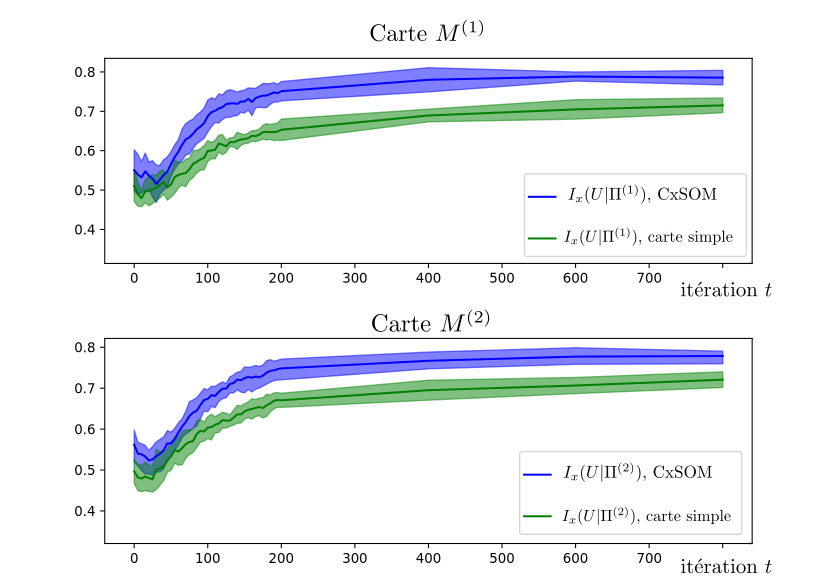
\includegraphics[width=\textwidth]{evolution_MI_binning}
\caption{Evolution du coefficient d'incertitude dans chaque carte au long de l'apprentissage. La courbe bleue correspond à $I_x(U|\bmu)$ dans l'architecture de cartes $M\m{1}$ et $M\m{2}$. On compare cette évolution à l'évolution de l'information d'une seule carte apprenant sur les mêmes entrées $X$ ou $Y$, sans être connectée.}
\label{fig:MI_evol}
\end{figure}

\subsection{Discussion}
\subsubsection{Influence de l'estimation}
Lorsque la dimension augmente, le nombre d'échantillon disponibles doit augmenter exponentiellement avec la dimension des variables pour éviter le phénomène de "boîtes vides": à cause de la dispersion des données, de nombreuses boîte $(x_j,y_i)$ ne contiendront pas de points alors qu'elles auraient du en contenir selon leur distribution; l'estimation de la probabilité en ce point sera donc nulle, et l'estimation faussée. 

Nous avons donc envisagé d'autres estimateurs moins biaisés en grand dimension. Détaillons par exemple l'estimateur par KNN (K-nearest neighbors) de Kraskov \cite{2004kraskov}. 
Cet estimateur ne passe pas par l'estimation de la densité de probabilité, contrairement aux histogrammes, mais estime directement l'information mutuelle. C'est l'estimation de la densité de probabilité qui posai justement problème en grande dimension.
Le découpage de l'espace se fait en recherchant, pour un couple $(X,Y)$ les k plus proches voisins. Une information mutuelle locale est calculée dans cette zone de l'espace, suivant une formule permettant d'approximer les différences de logarithme par la fonction digamma $\psi$ : 
$$i_j(X,Y) = \psi(k) - \psi(n_{x_j} + 1) - \psi(n_{y_j} +1) + \psi(N)$$
Cette information mutuelle locale est ensuite moyennée sur l'ensemble des points: 
$$\hat{I}(X,Y) = \psi(k) - \langle\psi(n_{x_j} + 1) + \psi(n_{y_j} +1)\rangle + \psi(N)$$
Pour estimer $I_x(X|Y)$, on estimera $I(X,Y)$ et $H(Y)$ avec les mêmes paramètres, en notant que $H(Y) = I(Y,Y)$.

Comparons les deux méthodes d'estimation de l'information mutuelle proposées dans ce chapitre: l'estimation par histogrammes, et l'estimation par KNN de Kraskov.
En figure~\ref{fig:MI_evol_total}, nous tracons l'évolution de l'information mutuelle moyenne, cette fois estimée par la méthode de Kraskov. Sur le même schéma, nous tracons également l'évolution de l'information mutuelle obtenue par la méthode des histogrammes. 

Sur les tracés, l'indicateur calculé avec la méthode de Kraskov converge vers une même valeur à la fin de l'apprentissage pour la carte simple que pour la carte au sein d'une architecture CxSOM (tracés rouges et noirs). Ce résultat est étonnant: cela signifie donc que la carte au sein de CxSOM n'a pas plus d'information sur le modèle que la carte isolée, lorsque cette information est estimée avec la méthode de Kraskov. Ce résultat va également à l'encontre de ce qu'on observe sur l'évolution de l'information mutuelle calculée par les histogrammes, dans laquelle une différence franche est observée entre la carte isolée et la carte au sein de l'architecture.

Proposons une explication.
La méthode des noyaux de Kraskov est plus "granulaire" que la méthode des histogrammes au niveau de l'estimation, c'est à dire que les données sont considérées \emph{points par point}. L'avantage est que l'évaluation de la relation fonctionnelle entre $U$ et $\bmu\m{i}$ est plus précise qu'avec les histogrammes: s'il y a deux valeurs de $U$ pour un même $\bmu\m{i}$, l'information diminue. Par contre, la contribution de ces deux valeurs sera la même dans le calcul de l'information mutuelle, qu'elles soient proches ou éloignées: la distance entre donnée n'intervient pas dans le calcul. Cette différence de contribution est illustrée en figure~\ref{fig:exemple-limite}. On calcule l'information mutuelle $I_x$ dans les deux cas de distribution proposées, à l'aide de l'estimateur granulaire de Kraskov. Dans le cas ou la relation est proche d'une relation fonctionnelle, mais est très bruitée, l'information $I_x(Y|X)$ est plus faible que dans le cas ou cette relation n'est pas fonctionnelle, mais sans bruit parasite.

On observe que l'information $I_x(U|\bmu)$ tend vers une même valeur dans CxSOM et dans une carte isolée quand on la calcule avec l'estimateur granulaire. Cela signifie, qu'on a la même quantité d'information sur $U$ avec le BMU, dans la carte isolée que dans CxSOM. Simplement, cette information n'est pas répartie de la même façon. 
Dans une carte isolée, le niveau de quantification vectorielle qu'on effectue sur $X$ est très précis: lorsqu'on présente une entrée $X$ à la carte, le poids du BMU est très proche de cette valeur $X$ Dans CxSOM, on perd ce niveau de quantification, ce qu'on a observé en figure~\ref{fig:erreur}. Le fait que l'indicateur, lorsqu'il est estimé avec une méthode très granulaire, prend la même valeur dans les deux expériences traduit alors qu'on a perdu de l'information sur l'entrée $X$ par rapport à la carte isolée, avec la perte de précision, mais qu'on a gagné de l'information sur l'autre entrée $Y$. Le fait que les deux évolutions de $I_x$, pour chaque expérience, convergent vers la même valeur montre qu'on est dans une situation de compromis: on gagne de l'information sur le modèle au détriment de l'information sur l'entrée externe.

C'est donc le fait de discrétiser grossièrement la distribution de $U$ qui permet de mesurer le gain d'information sur le modèle complet, sans prendre en compte le fait que la précision sur l'entrée externe est affaiblie. L'indicateur $I_x$ reste un indicateur fiable, mais il doit être utilisé en prenant en compte cet aspect.

%ela a peu de sens dans le cas de notre application: on souhaite mesurer que $U$ est proche d'une fonction de $\bmu$, mais du bruit est toléré. L'estimation par histogrammes permet de ne pas prendre en compte ce bruit; ce n'est pas possible avec la méthode de Kraskov. 



\begin{figure}
    \centering
    \includegraphics[width=0.35\textwidth]{kraskov.pdf}
    \caption{Découpage en KNN de Kraskov pour estimer l'entropie et l'information mutuelle des variables $X$ et $Y$. Les plus proches voisins du point rouge sont trouvés, en vert, et le processus est répété sur tous les points. Les valeurs de $n_x$ et $n_y$ permettent d'estimer directement l'entropie.}
    \label{fig:kraskov}
\end{figure}

\begin{figure}
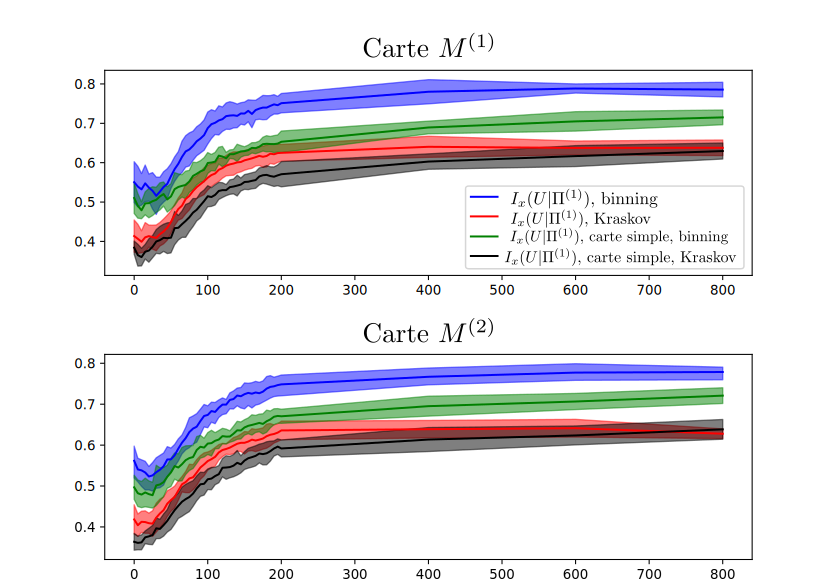
\includegraphics[width=\textwidth]{evolution_MI}
\caption{Evolution du coefficient d'incertitude dans chaque carte au long de l'apprentissage, en comparant l'estimation par histogrammes et l'estimation par la méthode de Kraskov.}
\label{fig:MI_evol_total}
\end{figure}

\begin{figure}
    \centering
    \includegraphics[width=\textwidth]{comparaison_binning_kraskov.pdf}
    \caption{Comparaison du calcul de l'indicateur $I_x$ sur deux distributions. A gauche, la relation entre $Y$ et $X$ se rapproche d'une fonction, mais bruitée. A droite, la relation n'est pas fonctionnelle, mais de telle sorte qu'une valeur de $X$ correspond au maximum à deux valeurs de $Y$. Lorsqu'on calcule l'indicateur avec la méthode très granulaire de Kraskov, cet indicateur est plus élevé dans le cas de droite que de gauche: en effet, le calcul ne prend pas en compte si les points sont condensés ou éloignés. Pour que l'indicateur nous informe correctement sur l'aspect fonctionnel de la relation entre $X$ et $Y$, il faut enlever manuellement le bruit. Avec la méthode par histogrammes, on prend une taille de boîte de $0.1$ selon $Y$. Dans ce cas, l'indicateur est bien plus élevé à gauche, ou $Y$ se rapproche d'une fonction de $X$, que à droite.}
    \label{fig:exemple-limite}
    \end{figure}

\subsubsection{Perspectives}

L'indicateur que nous proposons, $I_x(Y|X) = \frac{I(X,Y)}{H(Y)}$ traduit bien le fait que les cartes ont appris une relation entre les entrées. Son estimation doit passer par une discrétisation avec des intervalles larges pour $U$, afin de ne pas prendre en compte la perte d'information sur l'entrée externe $X$.
Les données doivent égalemement être débruitées avant l'estimation.
L'information mutuelle et l'entropie étant des quantités fondamentales en théorie de l'information, il existe de nombreuses méthodes d'estimations de ces valeurs malgré la difficulté qu'elle pose, voir~\cite{Doquire2012ACO} pour une revue de différentes méthodes. Ainsi, l'utilisation du coefficient d'incertitude comme indicateur reste robuste pour des données de plus grande dimension ou pour plus de cartes, en utilisant des méthode d'estimations plus élaborées. Cependant, cette estimation devra être retravaillée en plus grande dimension. 

\draft{
Une solution serait par exemple de chercher à séparer les sources d'information: l'information apportée par $X$ sur $U$ de l'information apportée par $\bmu$ sur $U$. On pourrait alors mesurer un gain d'information. Par exemple, en~\cite{williams_nonnegative_2010}, les auteurs décomposent l'information à plusieurs variables en \emph{redondance} et \emph{synergie}. 
}


% \draft{
% \subsection{Autre indicateur: le ratio de core}

% L'indicateur correlation ration permet de mesurer la distance d'une distribution à la fonction qui la fitte. Cela correspond bien à ce qu'on cherche dans CxSOM, mais estimation complexe aussi en grand dimension. 
% }

\section{Conclusion}
\begin{itemize}
\item La représentation par échantillonnage et variable aléatoire permet de mieux comprendre les mécanismes des cartes, ceux ci ne reposant plus directement sur les courbes de poids
\item Ces tracés montrent qu'une architecture de deux cartes s'organise comme une carte simple, mais modulée par l'entrée contextuelle: les poids externes se déplient comme une carte simple, mais les poids contextuels amènent des zones dans la carte. Ces zones séparent les BMUs en fonction de à la fois les entrées externes (organisation générale), et des entrées contextuelles (localement). Observation d'un nombre réduit de zones. 
\item Perte de précision au niveau de la quantification des poids externes, mais apprentissage d'un modèle. Nécessité de faire un compromis, réalisé de façon auto-organisée. Chaque carte a alors appris le modèle en entier et non seulement son entrée.
\item Utilisation d'un indicateur basé sur l'info mutuelle pour évaluer comment une carte apprend le modèle. Indicateur pouvant être utile en grande dimension ; mais l'estimation peut poser problème à ce moment.
\end{itemize}


\comment{Correlation ration : mesure de dépendance fonctionnelle
Débruitage de l'IM : répétition de l'expérience et moyenne ?}
\draft{Le ration de corrélation traduit mieux que le coefficient d'incertitude la dépendance fonctionnelle entre le modèle et le BMU. Cependant, à l'inverse de l'information mutuelle, une relation non fonctionnelle mais précise (telle que l'exemple du cercle de la figure~\ref{fig:exemple-limite}) entre les variables aura un score très faible. Ce n'est pas non plus voulu. 

Il semble que l'information mutuelle reste le moyen le plus prometteur et le plus général de mesurer la relation entre les éléments des cartes. Dans le cas une dimension, on observe qu'on veut tendre vers U fonction du BMU; on connait mal le comportement recherché en dimension plus grande (cartes 2D, entrées de grande dimension). L'information mutuelle laisse donc l'opportunité à plus d'états d'organisation des cartes de l'architecture d'avoir un bon score. La meilleure perspective serait donc de pouvoir calculer le coefficient d'incertitude sur des échantillons provenant de données non bruitées, ou de pouvoir séparer le bruit des données lors du calcul du coefficient.
Dans cette optique, l'estimateur par histogrammes permet de réduire l'effet du bruit, en choisissant correctement les tailles de boîtes. L'utilisation histo versus Kraskov reste donc à discuter.
Dans le cas ou le modèle d'entrée est connu, calculer les réponses des cartes sur des jeux de données non bruitées générées artificiellement, après apprentissage sur un jeu de données réelles et bruitée, est une solution. Si le modèle n'est pas connu, des méthodes statistique de réduction de bruit peuvent être imaginées.} 

\draft{
\section{Prédiction d'entrée}

Au sein d'une architecture de cartes, il est possible de ne pas présenter à une ou plusieurs cartes de l'architecture leur entrée externe $\inpx\m{i}$. Dans ce cas, une best matching unit peut quand même être calculée par leurs entrées contextuelles. Le poids de cette best matching unit peut alors être vu comme une prédiction de l'entrée manquante. Cette capacité de prédiction peut être à la fois vue comme une application possible de l'architecture, mais aussi comme une façon de représenter \emph{ce que les autre cartes connaissent d'une autre}. Tracer les prédictions d'une carte est donc un indicateur de la façon dont une architecture a appris des relations. 


\comment{
2 parties dans estimation/perspectives : 
d'une part, questionnement sur l'estimation des données bruitées par exemple - pas besoin de proposer des solutions si elles ne sont pas testées ? 
Et parler de l'estimation en grande dimension : ce n'est pas forcément le pb ici. Donc pas la peine...
}
}

\chapter{Analyse}

\section{Analyse de la relaxation}
\graphicspath{{04-Analyse/}}
\minitoc
Le processus de relaxation utilisé dans l'algorithme CxSOM est une méthode originale pour construire des connexions bidirectionnelles entre cartes. Deux cartes connectées de cette façon jouent alors un rôle symétrique, contrairement à une connexion unidirectionnelle ou hiérafchique ou une carte joue le rôle d'entrée. Dans cette section, nous évaluons expérimentalement la méthode de relaxation en tant que moyen de trouver une Best Matching Unit cohérente. On cherchera notamment à répondre aux questions suivantes :  
\begin{itemize}
\item Est-ce que la méthode de relaxation converge ?
\item Est-ce que que cette méthode est déterministe ?
\item Quels sont les paramètres à prendre en compte dans l'algorithme de relaxation ?
\end{itemize}

\subsection{Formalisation de la relaxation}

La relaxation est une recherche de point fixe de l'activité globale de chaque carte de l'architecture. Notons $(\mathbf{\bmu})_\tau = (\bmu\m{0}_\tau,\cdots,\bmu\m{N}_\tau)$ la suite définie par l'évolution des BMUs des $N$ cartes d'une architecture lors de la relaxation.
La suite $(\mathbf{\bmu})_\tau$ est une suite définie par récurrence par $\mathbf{\bmu}_{\tau+1} = \mathbf{f}(\mathbf{\bmu}_\tau)$
avec $\mathbf{f} = (f\m{0},\cdots,f\m{N}) : [0,1]^N \rightarrow [0,1]^N$ une application non linéaire transformant l'espace des positions des BMUs; $\mathbf{f}$ ne dépend pas de $\tau$.


Détaillons l'évolution de cette suite. Pour clarifier les notations, définissons pour chaque carte~$i$:
\begin{equation}
\begin{gathered}
p\star\m{i}_{\tau} = \argmax_{p\m{i}}(a_g\m{i}(p\m{i},\bmu\m{i_0}_\tau, \cdots \bmu\m{i_K}_\tau))\\
 i_0, \cdots i_K \: \text{indices des cartes nourrissant la carte $i$}.
\end{gathered}
\label{eq:pstar}
\end{equation}
$a_g\m{i}$ est une fonction des poids de la carte $\w\ext\m{i}, \w\cont\m{i}$ et de son entrée externe $\inpx\m{i}$. Lors du processus de relaxation, les poids et l'entrée restent fixes. Le calcul de $a_g$ ne dépend pas de $\tau$.
Pour toute carte $i$, $p\star\m{i}_{\tau}$ est donc seulement une fonction de $(\bmu\m{i_0}_\tau, \cdots \bmu\m{i_K}_\tau)$.
L'équation d'évolution s'écrit alors: 
\begin{equation}
\bmu\m{i}_{\tau+1} = 
\begin{cases}
\bmu\m{i}_{\tau} + sgn(p\star\m{i}_{\tau} - \bmu\m{i}_{\tau}) \times \delta \; & \text{si $p\star\m{i}_{\tau} - \bmu\m{i}_{\tau} > \delta$ } \\
p\star\m{i}_{\tau} \; \text{sinon}	
\end{cases}
\label{eq:evolution}
\end{equation}

En posant $f\m{i}$ la partie droite de l'équation \ref{eq:evolution}, on peut donc écrire: 
\begin{equation}
\bmu\m{i}_{\tau +1} = f\m{i}(\bmu\m{0}_\tau,\cdots,\bmu\m{N}_\tau)
\label{eq:fonction}
\end{equation}
Soit, pour l'ensemble des composantes : 
\begin{equation*}
\mathbf{\bmu}_{\tau+1} = \mathbf{f}(\mathbf{\bmu}_\tau)
\end{equation*}
L'état initial $(\bmu\m{0}_0, \cdots , \bmu\m{N}_0)$ est défini dans CxSOM par: 
\begin{equation}
\begin{cases}
\bmu\m{0}_0 = \argmax_{p\m{0}} a_e(p\m{0},\inpx\m{0})\\
\cdots \\
\bmu\m{N}_0 = \argmax_{p\m{N}} a_e(p\m{N},\inpx\m{N})\\
\end{cases}
\label{eq:init}
\end{equation}

La relaxation se traduit ainsi par une recherche de point fixe de la suite $(\mathbf{\bmu})_{\tau}$, soit une position $\mathbf{\bmu}$ telle que:
\begin{equation}
\mathbf{\bmu} = \mathbf{f}(\mathbf{\bmu})
\label{eq:suite}
\end{equation}

Si $f$ admet un point fixe, alors ce point fixe est aussi un point fixe pour la suite $(\mathbf{\bmu})_\tau$. Cependant, rien ne garantit que ce point fixe existe, et qu'il sera atteint par la suite.
Expérimentalement, il semble que si $\mathbf{f}$ admet un unique point fixe, alors $(\mathbf{\bmu})_{\tau}$ converge vers ce point fixe. On montrera que ce point fixe n'est pas toujours unique, notamment lorsque les poids sont aléatoires au début de l'apprentissage, ce qui entraîne alors une non-convergence de la relaxation. Cependant, ces cas de non-convergence n'influencent pas l'apprentissage des cartes en choissant des bons paramètres d'apprentissage. On observera expérimentalement qu'à la fin de l'apprentissage, la disposition des poids permet l'existence d'un unique point fixe. 


\subsection{Etude de la convergence des BMUs lors de la relaxation}

La méthode de relaxation cherche la convergence des BMUs de l'architectures. Nous avons donc réalisé 1000 itérations de test, à poids figés, à différents temps d'apprentissage, et comptons le nombre de pas nécessaires à la convergence de la relaxation. L'algorithme utilisé pour la relaxation s'arrête automatiquement si la relaxation dépasse $\tau_{max}= 1000$ itérations. On considérera que la relaxation n'a pas atteint un point de convergence si la relaxation atteint ces $\tau_{max}$ itérations.
Théoriquement, plusieurs situations se traduisent par une non-convergence de la relaxation:
\begin{itemize}
\item La relaxation évolue vers un point de convergence, mais trop lentement pour y arriver en moins de 1000 itérations
\item La relaxation évolue vers un cycle limite composé d'un nombre limité d'unités étant alternativement best matching units
\item La relaxation évolue sans répétition de motifs dans la carte : évolution chaotique.
\end{itemize}
Le premier cas est évité car la limite de 1000 itérations est assez grande par rapport à la taille de la carte, les cartes sont de tailles 500. Le pas d'évolution de la relaxation est d'une dizaine d'unités. La convergence, si elle existe, est donc rapide. Nous observerons plus précisément les trajectoires dans la section suivante; on s'intéresse ici seulement à la question de la convergence.
L'étude de la convergence sera réalisée dans des architectures de 2 et 3 cartes, pour des cartes une dimension et deux dimensions.

La figure \ref{fig:conv_evolution} présente l'évolution du taux de convergence au cours de l'apprentissage d'une architecture de 2 cartes et 3 cartes. La figure \ref{fig:conv_evolution2D} trace  cette évolution dans le cas ou les cartes sont en 2 dimensions. Pour tracer cette évolution, on effectue des étapes de tests à intervalles réguliers au cours de l'apprentissage, pendant lesquels les poids ne sont pas mis à jours. Ces tests sont réalisés sur 1000 entrées externes $X,Y$ (et $Z$ pour trois cartes), prises aléatoirement dans l'espace d'entrée. On prélève, pour chaque échantillon de test, le nombre de pas nécessaire à la relaxation. Si ce nombre est égal à $\tau_{max}$, on considère que la relaxation n'a pas convergé. On trace alors, en haut, le pourcentage d'échantillons de test pour lesquel la relaxation converge. En bas, on trace le nombre moyen de pas de relaxation nécessaires à la convergence.
Dans chaque cas, on répètera 10 fois l'apprentissage, et on trace la moyenne et écart type des valeurs obtenues sur ces 10 répétition.

Au début de l'apprentissage, lorsque les poids sont aléatoirement initialisés, la relaxation atteint rarement un point de convergence. Lorsque les cartes se déplient, la relaxation évolue vers un point de convergence dans plus de $90 \%$ des cas. Cette évolution est similaire pour des architecture de deux et trois cartes. Les expériences avec des cartes en deux dimensions présentent la même évolution. Le taux de convergence en fin d'apprentissage est plutot situé entre $80 \%$ et $90 \%$.
 
\begin{figure}
\centering
\includegraphics[width=0.7\textwidth]{1D_conv_evolution_total.pdf}
\caption{Evolution du taux de convergence moyen lors de la relaxation au cours de l'apprentissage sur deux et trois cartes 1D. Chaque point est calculé sur un échantillon de 1000 relaxations au temps t, évaluées sur des entrées différentes prises aléatoirement sur le cercle. Moyenne et écart-types calculés sur 10 expériences.}
\label{fig:conv_evolution}
\end{figure}


\begin{figure}
\centering
\includegraphics[width=0.7\textwidth]{2D_conv_evolution_total.pdf}
\caption{Evolution du taux de convergence moyen lors de la relaxation au cours de l'apprentissage sur deux et trois cartes 2D. Chaque point est calculé sur un échantillon de 1000 relaxations au temps t, évaluées sur des entrées différentes prises aléatoirement sur le cercle. Moyenne et écart-types calculés sur 10 expériences.}
\label{fig:conv_evolution2D}
\end{figure}

\subsection{Etude de l'influence de l'entrée contextuelle sur le BMU}

Dans cette section, nous étudions plus précisément l'évolution de la suite $(\mathbf{\bmu})_{\tau}$ dans le cas de d'une architecture de deux cartes connectées. Les cartes sont $M\m{1}$ et $M\m{2}$ prenant en entrée externe respectivement $\inpx\m{1} = X, \inpx\m{2} = Y$.
Les entrées contextuelles des deux cartes sont à valeurs dans l'espace des positions d'une carte: $\inpc\m{1} = \bmu\m{2}$ et $\inpc\m{2} = \bmu\m{1}$
On définit donc les valeurs $p\star\m{1}$ et $p\star\m{2}$ comme indiqué dans l'équation \ref{eq:pstar}
\begin{equation} 
\begin{cases}
	p\star\m{1}_{\tau} = \argmax_{p\m{1}}(a_g(p\m{1},\bmu\m{2}_{\tau}) \\
	p\star\m{2}_{\tau} = \argmax_{p\m{2}}(a_g(p\m{2},\bmu\m{1}_{\tau}) \\
\end{cases}
\end{equation}

On tracera les valeurs de $p\star\m{1}$ en fonction de son entrée contextuelle $\bmu\m{2} \in [0,1]$, et $p\star\m{2}$ en fonction de $\bmu\m{1} \in [0,1]$ en figure \ref{fig:w006}.
Cette expérience est réalisée après l'apprentissage. On remarque que, $p\star\m{i}$ varie peu en fonction de l'entrée contextuelle de la carte; la relaxation se déroulera donc dans une partie réduite de la carte.

On peut comparer ces tracés à ceux réalisés au début de l'apprentissage ($t=0$), lorsque les poids sont aléatoires, et pendant l'apprentissage ($t=150$). Pour $t=150$, les poids externes ont déjà convergé, mais pas encore les poids contextuels, car le rayon de voisinage utilisé pour les poids contextuel est bien plus faible que pour les poids externes.
%TODO tracés (cercle 006)

\begin{figure}
\includegraphics[width=\textwidth]{am_w_006}
\caption{A gauche, $p\star\m{1}$ et $p\star\m{2}$ en fonction de l'entrée contextuelle de leur carte $\bmu\m{2}$ et $\bmu\m{1}$. A droite, les poids externes et contextuels des cartes $1$ et $2$ sont représentés selon leur position dans la carte. On représente également les entrées test $\inpx\m{1}$ et $\inpx\m{2}$ en fonction de leur BMU. Les entrées utilisées pour tracer les figures de gauche sont colorées en rouge sur les figure de droite: $\inpx\m{1}=0.26,\inpx\m{2}=0.06$}
\label{fig:w006}
\end{figure}

En figure \ref{fig:diff_relax} et \ref{diff_relax_t1}, nous représentons les valeurs $\lvert p\star\m{1} - p\m{1} \rvert$ et $\lvert p\star\m{2} - p\m{2}\rvert$ en fonction de $p\m{1},p\m{2} \in [0,1]$. On rappelle que $p\star\m{1}$ dépend de $p\m{2}$, et inversement.
Le point fixe, s'il existe, est alors à une position $p\m{1},p\m{2}$ vérifiant:
\begin{equation*}
\begin{cases}
p\star\m{1}(p\m{2}) = p\m{1}\\
p\star\m{2}(p\m{1}) = p\m{2}\\
\end{cases}
\end{equation*}

A la fin de l'apprentissage, ce qui est le cas en figure \ref{fig:diff_relax}, un point fixe semble exister.

\subsection{Etude de l'unicité du point fixe}

Nous étudions dans cette partie l'évolution de processus de relaxation lancés sur les mêmes poids, pour une entrée externe fixée, mais avec $\mathbf{\bmu}_0$ intialisés à des valeurs aléatoires dans chaque carte.
\draft{Chacun de ces processus aboutit sur un point de convergence; on tracera donc la distance moyenne entre les différents points de convergence sur toutes les expériences. Si cette distance est nulle, alors le point de convergence est un point fixe qui ne dépend pas de l'initialisation. 
Cette étude sera réalisée sur des cartes 1D et 2D, pour des architectures de 2 et trois cartes.}

\begin{figure}
\begin{minipage}{0.5\textwidth}
\centering
\includegraphics[width=\textwidth]{champ_X_006.pdf}
\end{minipage}
\begin{minipage}{0.5\textwidth}
\centering
\includegraphics[width=\textwidth]{champ_Y_006.pdf}
\end{minipage}
\caption{Valeur de ${p\star}\m{1} - p\m{1}$, resp. ${p\star}\m{2} - p\m{2}$. ${p\star}\m{1}$ ne dépend que de $p\m{2}$ : on peut donc tracer cette valeur selon deux dimensions pour chaque carte. Les zones où cette valeur est nulle sont en violet sur le graphique. Les points fixes, s'il existent, sont aux positions de différence nulle pour $M\m{1}$ et $M\m{2}$.}
\label{fig:diff_relax}
\end{figure}

\begin{figure}
\begin{minipage}{0.5\textwidth}
\centering
\includegraphics[width=\textwidth]{champ_X_006_t1.pdf}
\end{minipage}
\begin{minipage}{0.5\textwidth}
\centering
\includegraphics[width=\textwidth]{champ_Y_006_t1.pdf}
\end{minipage}
\caption{Valeur de ${p\star}\m{1} - p\m{1}$, resp. ${p\star}\m{2} - p\m{2}$. ${p\star}\m{1}$ ne dépend que de $p\m{2}$ : on peut donc tracer cette valeur selon deux dimensions pour chaque carte. Les zones où cette valeur est nulle sont en violet sur le graphique. Les points fixes, s'il existent, sont aux positions de différence nulle pour $M\m{1}$ et $M\m{2}$.}
\label{fig:diff_relax_t1}
\end{figure}

\begin{figure}
\centering
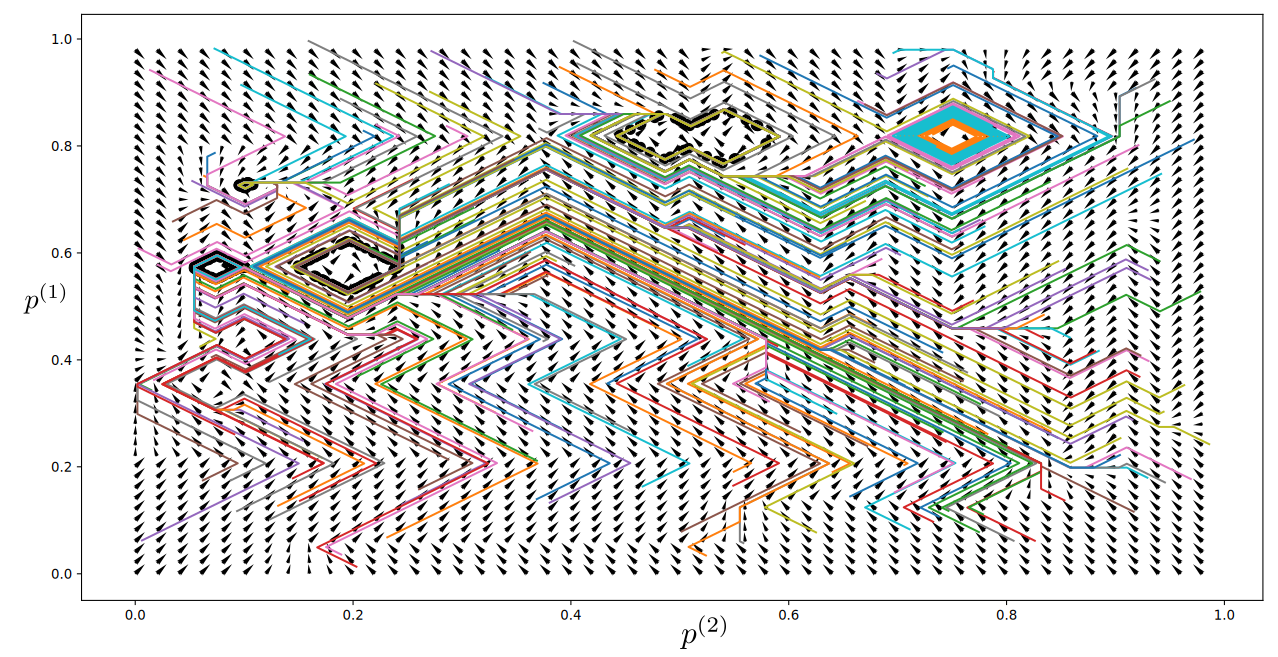
\includegraphics[width=\textwidth]{champ_006_t1.pdf}
\caption{Champ de déplacements de $\bmu\m{1},\bmu\m{2}$ lorsque les poids sont encore aléatoires, à $t=0$. En fonction de la position initiale des BMUs, la relaxation évolue vers un point fixe ou un cycle limite.}
\label{fig:champ_0}
\end{figure}


\begin{figure}
\centering
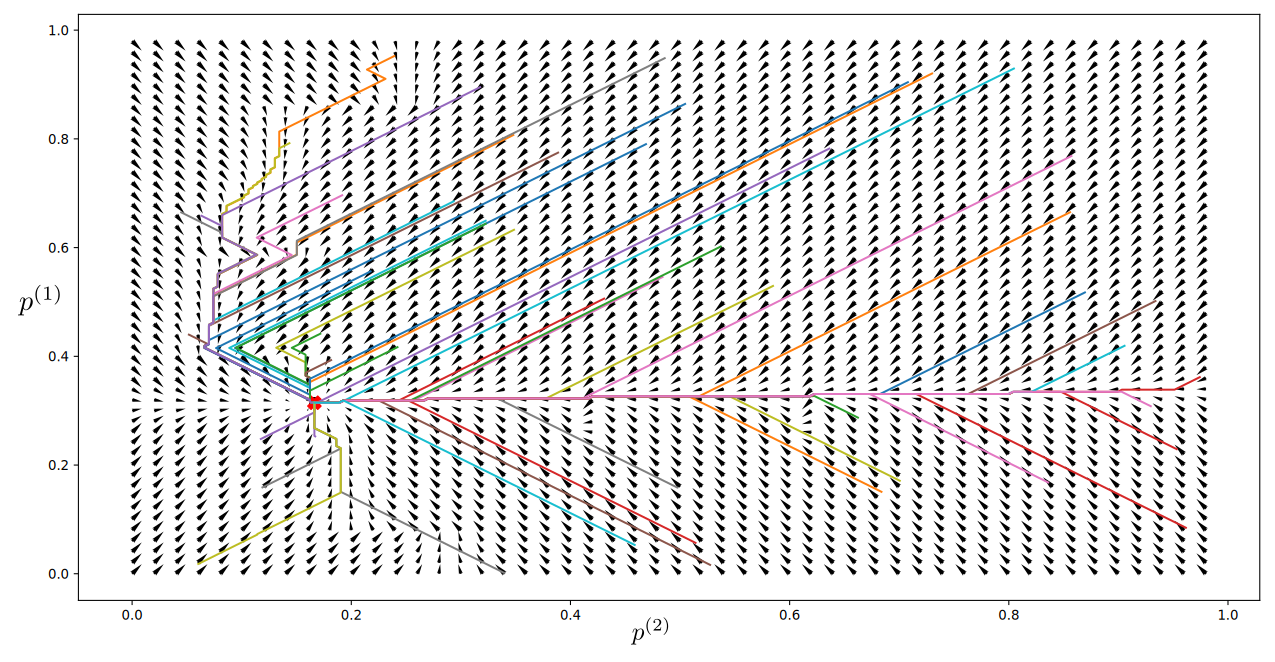
\includegraphics[width=\textwidth]{champ_006.pdf}
\caption{Champ de déplacements de $\bmu\m{1},\bmu\m{2}$ lorsque les poids sont organisés tels que représentés en figure \ref{fig:am_w_006}, à $t=9999$. La relaxation évolue vers un point fixe pour l'entrée considérée.}
\label{fig:champ_9999}
\end{figure}

\subsection{Influence du pas de convergence}

Dans les expériences précédentes, on a utilisé un pas de convergence $\delta=0.05$. On peut aussi ne pas utiliser de pas de relaxation, c'est à dire, à chaque itération, déplacer le BMU $\bmu\m{i}$ directement à la position ou l'activité globale est maximale, au lieu de le déplacer de $\delta$ vers cette position.
L'évolution de la relaxation devient alors:
\begin{equation}
\forall i, \bmu\m{i}_{\tau+1} = p\star\m{i}_{\tau}
\end{equation}
L'apprentissage est alors similaire

\draft{
\begin{itemize}
\item Convergence plus rapide quand ca converge
\item Potentiellement plus de risque de non convergence ( ? )
\item Même comportement d'apprentissage que sans relax = si point fixe, on tombe sur le même.
\end{itemize}
}

\subsection{Discussion}

\draft{
\begin{itemize}
\item Element clé de l'architecture : relaxation. A t-on toujours un point de convergence ? Sinon, dans quels cas ? 
\item On peut tracer les champs de relaxation pour trouver le point fixe. 
\item Une carte est un système dynamique comme une variable passant d'un état à un autre. Etat = BMU.
\end{itemize}
}


\section{Analyse de l'auto-organisation}
\chapter{Application à la prédiction d'entrée manquante}
\section*{Conclusion}



Perspectives : 

Mémoire associative pas forcément le cas d'étude le plus adapté à un contexte de modularité.
Mémoires temporelles (référence to Fred), interactions avec environnement vs modules d'apprentissage, \cite{Ellefsen2015NeuralMH}
Apprentissage sur le long terme.

Proximité avec modules récurrents pour une généralisation du modèle.
Perspective : envisager d'autres cas d'utilisation du modèle, qui induisent d'autres architectures.
%Bibliography files
\bibliography{01-Modularite/biblio_modularite.bib,01-Modularite/biblio_reseaux.bib, 03-Representation/biblio_representation.bib,02-SOM/biblio_SOM.bib}

\bibliographystyle{plain}
\end{document}